\chapter{血栓性疾病}

\section{前沿学术综述}

\subsubsection{静脉血栓栓塞症诊治的历史回顾与诊治现状}

静脉血栓栓塞症(venous
thromboembolism,VTE)是危及人们健康的常见疾病。对血栓和肺血栓栓塞的临床描述最早见于18世纪,1858年德国病理学家Rudolph
Virchow提出静脉血栓形成的三大机制:血液淤滞、血液高凝和血管壁损伤,迄今仍是指导临床工作的经典理论。治疗上,血栓切除术或者静脉结扎术是当时为数不多的手段。上世纪30年代静脉血栓栓塞症的治疗出现转机,1937年,Crafoord首次报道肝素可预防静脉血栓栓塞症,1938年Murray报道肝素用于静脉血栓栓塞症的治疗,1960年Barritt与Jordan发表了肝素治疗肺血栓栓塞症(pulmonary
thromboembolism,PTE)的对照研究,静脉滴注肝素加口服维生素K拮抗剂组的病死率和复发率仅为0和2%,而对照组分别为26%和52%,自此抗凝治疗成为静脉血栓栓塞症的标准疗法。1973年和1974年尿激酶与链激酶治疗肺血栓栓塞症的临床对照研究相继发表,为肺血栓栓塞症的治疗提供了更多的选择。诊断方面,20世纪60年代后,血管造影、肺核素通气/灌注显像以及超声影像等的应用提高了静脉血栓栓塞症的检出率和确诊率,血管造影迄今仍是静脉血栓栓塞症诊断的金标准。1990年肺血栓栓塞诊断的前瞻性调查(PIOPED)报道肺核素通气/灌注显像并不是肺血栓栓塞症理想的诊断工具,77%的患者由于显像结果与临床诊断的不同而仍然需要行有创的肺血管造影。近20年来MRI和螺旋CT血管造影技术以及血清标志物检查的出现则使静脉血栓栓塞症、尤其是肺血栓栓塞症的诊断水平出现了革命性的改变,血清标志物D-D二聚体成为静脉血栓栓塞症筛查的常规指标,螺旋CT血管造影技术已取代传统的血管造影技术成为临床确诊静脉血栓栓塞症的一线选择。2006年PIOPEDⅡ发表,重点评价了多层CT(MDCT,4~16排)肺血管造影联合盆腔和股静脉CT造影在肺血栓栓塞症诊断中的价值。研究提示肺血管造影诊断肺血栓栓塞症的特异性为96%,敏感性为83%;肺血管造影股静脉CT造影诊断的特异性为95%,敏感性为90%,从而证实肺血管造影和肺血管造影股静脉CT造影诊断肺血栓栓塞症的价值优于传统的肺通气/灌注显像。随着多层(16~128排)螺旋CT的发展和普及,此检查已成为肺血栓栓塞症诊断策略的核心。2010年PIOPEDⅢ完成,对增强的MRI肺动脉造影和静脉造影诊断肺血栓栓塞症的价值也做了评价,极大地丰富了当代肺血栓栓塞症的诊断手段。

急性静脉血栓栓塞症的抗凝治疗,除普通肝素外,低分子量肝素的出现给血栓栓塞性疾病的治疗带来了巨大变革。随着低分子肝素在各种血栓性疾病的大规模临床研究证据的不断积累,在许多领域低分子肝素已经或即将取代普通肝素。2004年美国胸科医师协会(ACCP)第7次抗凝与溶栓会议指南中,低分子肝素在各适应证中的推荐等级明显提高
\protect\hyperlink{text00022.htmlux5cux23ch1-21}{\textsuperscript{{[}1{]}}}
,可以说血栓栓塞疾病的防治迎来了低分子肝素时代。2008年6月该指南的第8版颁布,代表了国际抗凝与溶栓的最新进展和总结。同时,新一代的抗凝药物------直接凝血酶抑制剂如达比加群(dabigatran),口服的凝血因子Ⅹa抑制剂利伐沙班(rivaroxaban)、阿哌沙班(apixaban),同样具有选择性抑制凝血因子Ⅹa活性的磺达肝癸钠(fondaparinux)及其超甲基化衍生物依达肝素(idraparinux)或生物素化依达肝素(biotinylated
idraparinux)等新型抗栓药物也开始广泛应用于临床。溶栓治疗方面,第二代溶栓药物------重组组织型纤溶酶原激活物(rt-PA)的疗效明显优于尿激酶和链激酶作用。新型溶栓剂还包括组织型纤溶酶原激活物变异体(reteplase,r-PA)、重组单链尿激酶纤维蛋白溶酶原激活剂(rscu-PA)等,具有溶栓效果更快、无免疫原性等特点。除抗凝与溶栓药物之外,静脉血栓栓塞症的治疗手段还包括下腔静脉滤器、肺动脉血栓切除术和介入取栓术。慢性血栓栓塞性肺动脉高压(chronicity
thromboembolic pulmonary
hypertension)则可以选择药物保守治疗、肺动脉血栓切除术或肺移植。由此可见,当代静脉血栓栓塞症的诊断、治疗已形成完整的体系,静脉血栓栓塞症的检出率大大提高,病死率降低或生存质量改善(表\ref{tab16-1})
\protect\hyperlink{text00022.htmlux5cux23ch2-21}{\textsuperscript{{[}2{]}}}
。

\begin{table}[htbp]
\centering
\caption{静脉血栓栓塞症预防与治疗的历史回顾}
\label{tab16-1}
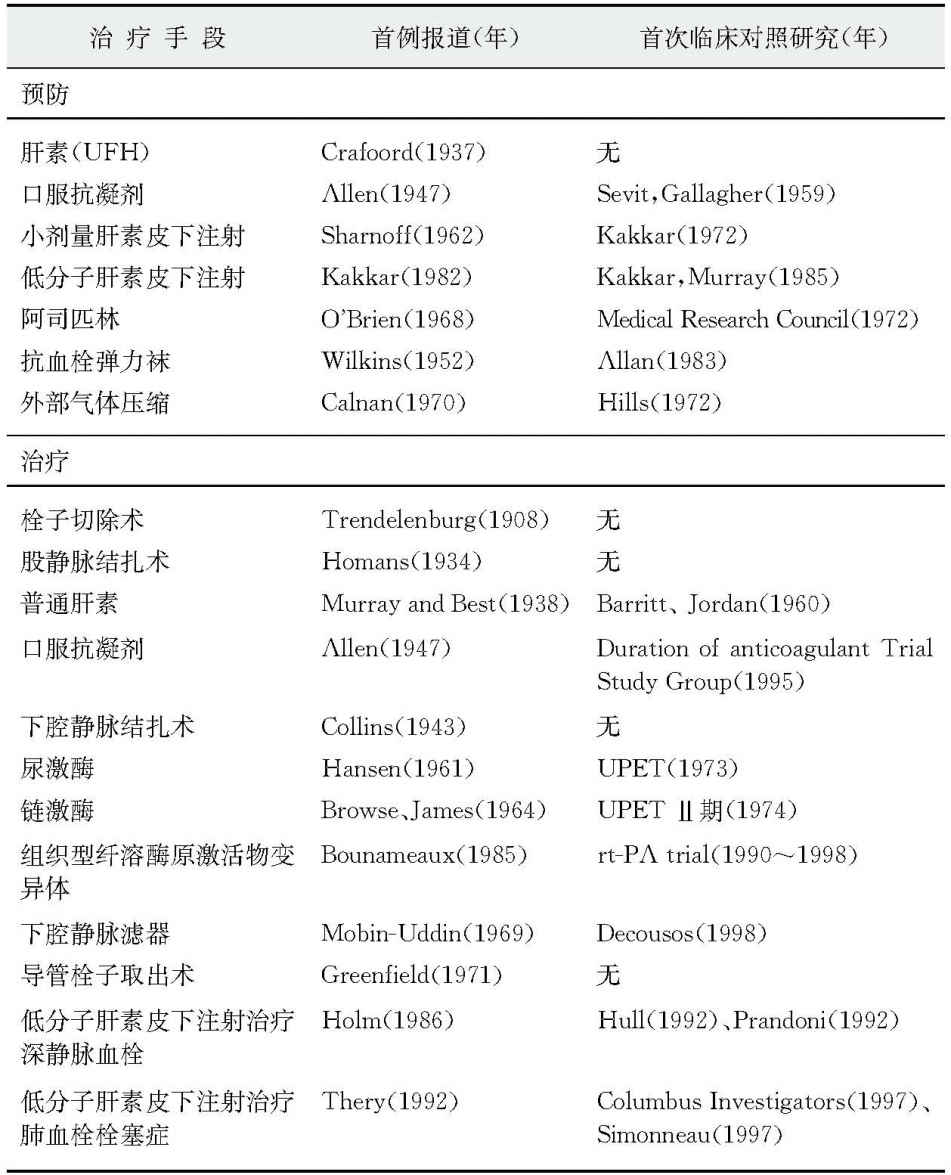
\includegraphics[width=\textwidth,height=\textheight,keepaspectratio]{./images/Image00116.jpg}
\end{table}

在我国,过去传统观念一直认为静脉血栓栓塞症,尤其是肺血栓栓塞症是少见病,因此认识普遍不足。尽管目前尚缺乏全国性的统计资料,但从近年来国内多家单位的联合调查以及肺血栓栓塞症检出率数十倍的增长趋势来看,肺血栓栓塞症绝非少见疾病。因此,需要大力提高对该病的临床警惕性,避免延误诊治。2001年中华医学会呼吸病学分会颁布了《肺血栓栓塞症的诊断与治疗指南(草案)》,随后国内开展了多项与流行病学、抗凝或溶栓有关的多中心研究,从而有效地提高了国内静脉血栓栓塞症的诊治水平,并为开创具有本国特色的静脉血栓栓塞症诊治方案进行了有益的尝试。

\subsubsection{目前存在的问题与前景}

临床上对静脉血栓栓塞症关注度如此之高的主要原因,就在于组成静脉血栓栓塞症的深静脉血栓形成(deep
venous
thrombosis)和肺血栓栓塞症临床表现隐匿或迁延、病情变化急骤,如不能及时诊断和治疗后果严重,随时危及生命。一项2388例普通住院人群的尸检报告显示,院内死亡的患者中,死因为肺血栓栓塞症者约10%,其中83%有下肢深静脉血栓,但只有19%的患者生前报告了下肢深静脉血栓症状,仅有3%的患者进行了相应的检查
\protect\hyperlink{text00022.htmlux5cux23ch3-21}{\textsuperscript{{[}3{]}}}
。尽管当代静脉血栓栓塞症的诊治领域不断有新的研究进展成果出现,但流行病学资料显示,近半个世纪以来,静脉血栓栓塞症的病死率并未明显减少,肺血栓栓塞症的病死率甚至还高于急性心肌梗死;静脉血栓栓塞症的误诊方面也有统计数据显示问题的严重性。这提示医学界需对现有静脉血栓栓塞症诊治模式进行检讨,并继续以前瞻性的大样本研究为基础积极寻找新的诊治方案。

造成静脉血栓栓塞症早期确诊率与治疗率低下而病死率高的原因在于,首先,静脉血栓栓塞症涉及范围广、表现复杂,因基础疾病的不同,易患因素与临床表现也各异,诊断与治疗也各有倾向性,难以全面把握;其次,已知静脉血栓栓塞症的临床表现缺乏特异性,确诊需要依靠辅助检查,尽管目前可供选择的检查设备颇多,但如何将首诊的临床判断与辅助检查有机地结合起来,以及如何根据静脉血栓栓塞症患者的来源,比如门诊、急诊或住院的疑似患者,构建相应的成本---效益比(cost-effctive),获得最佳的诊查策略一直缺乏定论,这些均是有待深入探讨的领域;第三,如何平衡抗凝与溶栓治疗的疗效与出血并发症的风险始终是临床决策的难点。此外,急性肺血栓栓塞症治疗上目前最有争议的领域在于溶栓对象的选择,对血压正常但超声心动图出现右室功能障碍(right
ventricular
dysfunction)的次大面积肺血栓栓塞症患者是否给予溶栓一直存在争议,这也需要进一步的国际研究和共识。治疗领域有待探讨的问题还包括,外科手术治疗与介入治疗的地位与价值、下腔静脉滤器的评价以及慢性血栓栓塞性肺动脉高压的综合治疗等。

纵观当代静脉血栓栓塞症的诊治现状,从易患因素的筛查及其临床意义到各种诊断手段的评估以及治疗方案的探讨,几乎每一处细节都有值得推敲的疑点或争议。以创伤患者静脉血栓栓塞症的预防为例,美国哈佛大学麻省总院创伤外科主任Velmahaos
\protect\hyperlink{text00022.htmlux5cux23ch4-21}{\textsuperscript{{[}4{]}}}
认为,文献报道的创伤后静脉血栓栓塞症发生率为0.5%~45%,相差90倍,已经达到了可笑的地步;而已有的研究则充斥着相互矛盾的结论,甚至荟萃分析竟发现不予预防强于预防的证据。由此可见,缺乏高质量的创新研究仍是目前困扰临床决策的首要问题。我们期待这些问题的早日解决,并呼吁国内各级单位加强科研协作,以循证医疗的原则为基础,根据自身特点制定适合本地区的诊治指南,切实有效地提高静脉血栓栓塞症的诊治水平。

\section{临床问题}

\subsection{临床部分}

\subsubsection{何谓下肢深静脉血栓、肺血栓栓塞症、静脉血栓栓塞症?}

首先应该明确何谓“深静脉”?体循环静脉分深、浅两类,位于深筋膜深面或体腔内者为深静脉,浅静脉则位于皮下浅筋膜内,浅静脉最终均注入深静脉。以下肢静脉为例,下肢静脉有大隐静脉和小隐静脉,大隐静脉起自足背静脉网内侧,在腹股沟韧带附近进入深静脉------股静脉。小隐静脉则在腘窝穿过深筋膜进入腘静脉。

下肢深静脉血栓是指血液在深静脉系统内不正常地凝结,属静脉回流障碍性疾病,血栓形成以下肢多见。来自全身静脉系统的血栓可脱落或游离,并向近端移行,经上、下腔静脉进入右心系统,并最终阻塞肺动脉及其分支,形成以肺循环和呼吸功能障碍为主要表现的临床综合征,是为肺血栓栓塞症。由于下肢深静脉血栓与肺血栓栓塞症存在着极为密切的同源性或相关性,两者在病因、发病情况、治疗和预后等诸多方面具有共同的特性,因此现主张将下肢深静脉血栓与肺血栓栓塞症看作是同一疾病的两种不同临床表现,即所谓的静脉血栓栓塞症。

肺动脉发生栓塞后,若其支配区域的肺组织因血流受阻或中断而发生坏死,则称为肺梗死(pulmonary
infarction),多见于原有肺循环异常者或病情严重影响到肺组织的多重氧供者。如果血栓栓子长期、反复脱落至肺动脉内,血栓机化后可形成慢性肺动脉栓塞,并造成血栓栓塞性肺动脉高压(thromboembolic
pulmonary
hypertension),此期治疗非常棘手,缺乏有效的治疗措施,预后不佳。

此外,临床上还常以肺栓塞(pulmonary
embolism)代替上述的肺血栓栓塞症,主要是因为造成肺循环阻塞的栓子中90%为血栓栓子,故而两者常混淆。不过应该明确肺栓塞还包括有脂肪栓塞、羊水栓塞、空气栓塞或其他医源性栓子栓塞,因此笼统地将肺栓塞等同于肺血栓栓塞症是不科学的。

\subsubsection{静脉血栓栓塞症的易患因素(危险因素)有哪些?}

正如Virchow所说,凡是能够导致“血液淤滞、血液高凝和血管壁损伤”的病因,理论上都可成为静脉血栓栓塞症的易患因素。一般将静脉血栓栓塞症的易患因素分为先天性和获得性两种,可以说静脉血栓栓塞症是一个由先天性和获得性因素共同作用而导致的复杂疾病(表\ref{tab16-2})
\protect\hyperlink{text00022.htmlux5cux23ch5-21}{\textsuperscript{{[}5{]}}}
\textsuperscript{~}
\protect\hyperlink{text00022.htmlux5cux23ch7-21}{\textsuperscript{{[}7{]}}}
。

\begin{table}[htbp]
\centering
\caption{静脉血栓栓塞症的易患因素}
\label{tab16-2}
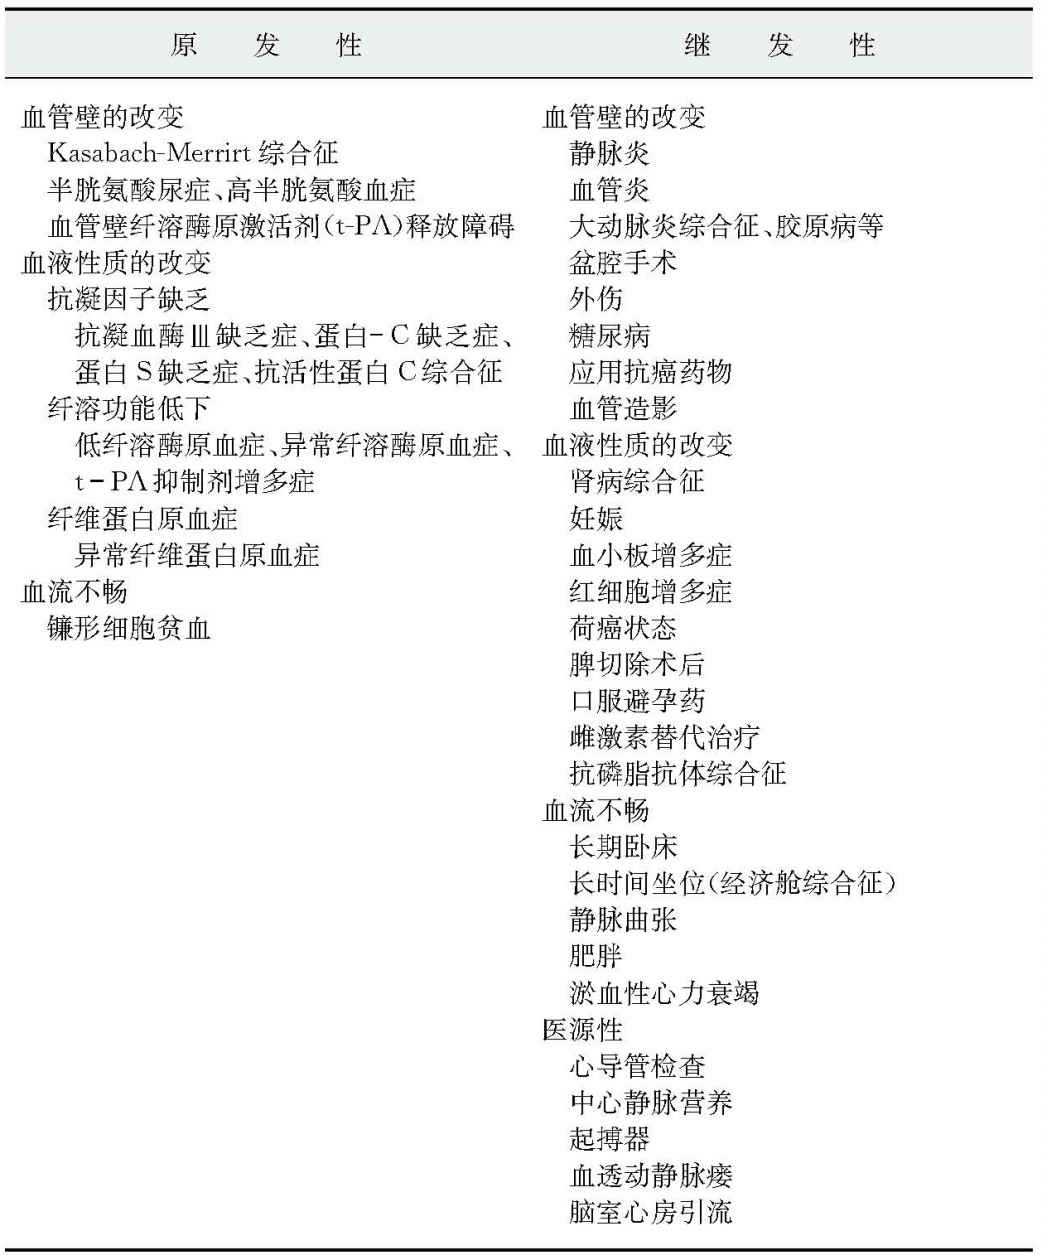
\includegraphics[width=\textwidth,height=\textheight,keepaspectratio]{./images/Image00117.jpg}
\end{table}

静脉血栓栓塞症先天性或原发性易患因素包括:Ⅴ因子Leiden变异(factor-Ⅴ
Leiden
mutation)、蛋白C缺乏、蛋白S缺乏、G20210A基因变异、抗凝血酶缺乏、抗磷脂抗体综合征和同型半胱氨酸血症等,常以反复静脉血栓栓塞或所谓的“易栓症(thrombphilia)”为主要临床表现。1993年报道的凝血因子Ⅴ基因变异打破了既往人们认为先天性凝血功能异常比较少见的看法------高加索人种中该变异基因携带者的比率高达3%~7%,在某些遗传性易栓症的家族中,该比率可达20%~60%。据估计该基因变异的杂合子发生血栓的危险性较无基因变异患者增加5~10倍,纯合子增至50~100倍。由于凝血因子Ⅴ基因第1691位核苷酸发生G→A突变,使翻译水平氨基酸序列的第506位由精氨酸变为谷氨酰胺,该位点正是活性蛋白C裂解的位点,故突变后的凝血因子Ⅴ虽表现出正常的促凝活性,但对活化蛋白C(APC)的分解不敏感,使得凝血活酶复合物稳定性增加,凝血酶产生速率增加导致血液高凝。也有报道认为该基因变异在非洲和亚洲罕见,因此在非高加索人种中凝血因子Ⅴ基因变异不是血栓形成的主要易患因素。对于凝血因子Ⅴ基因变异与其他易患因素的相互作用,以及是否需要对静脉血栓栓塞症患者进行易栓症普查尚在进一步研究之中。

获得性或继发性易患因素则较多,包括高龄、吸烟、肥胖、长途旅行、恶性疾病、血栓性静脉炎、静脉曲张、近期手术、全身性感染、创伤、心肺或神经系统疾病、既往血栓病史、长期制动或卧床、服用避孕药或雌激素等。在获得性易患因素中,外科手术是最值得重视的环节。术后静脉血栓栓塞症的危险性根据手术类型、是否合并其他易患因素可以分为低、中、高三类。对于不易发生血栓形成的择期手术患者,致死性肺血栓栓塞症的发生率仅为万分之一,而对较易发生血栓的下肢矫形手术、全腹或盆腔肿瘤手术,其近端静脉血栓的发生率可达10%~30%,致死性肺血栓栓塞症的发生率可达5%(表\ref{tab16-3}、表\ref{tab16-4})。非手术患者中,患心、肺、脑三大系统的急、慢性疾病以及恶性肿瘤患者属于高危人群,心肌梗死、脑卒中以及重症患者发生下肢深静脉血栓的风险分别为17%~34%、11%~75%和25%~42%。

\begin{table}[htbp]
\centering
\caption{外科手术患者的静脉血栓栓塞症的易患因素}
\label{tab16-3}
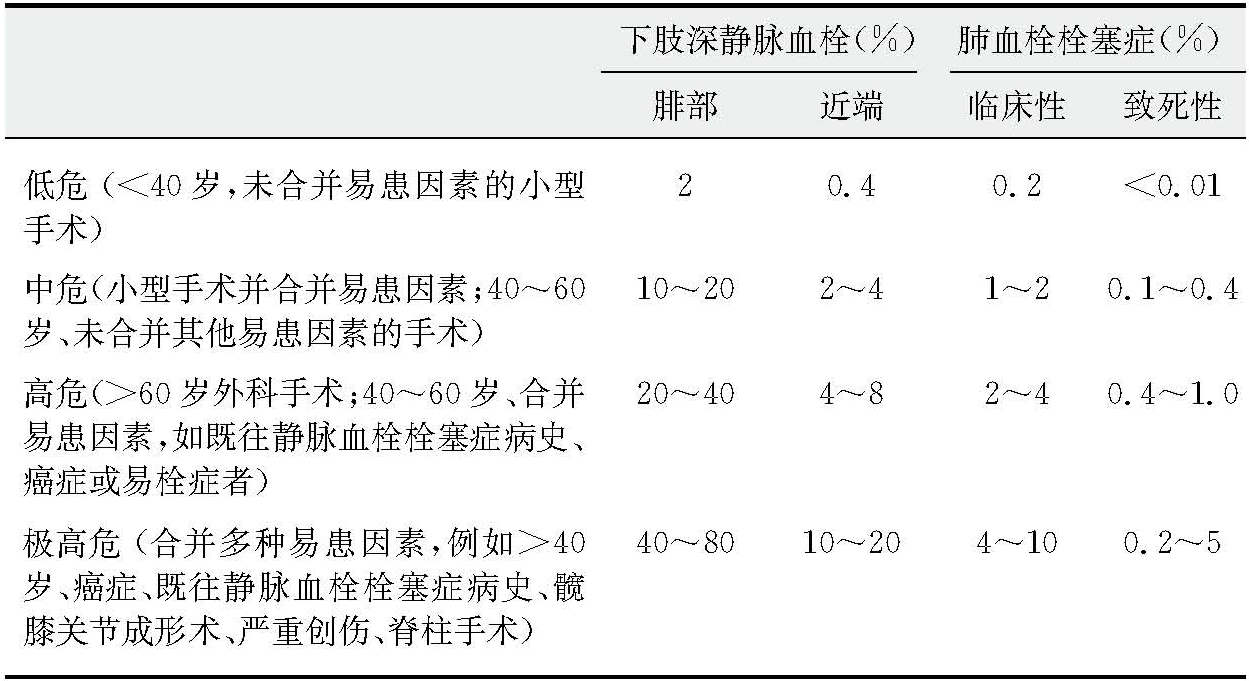
\includegraphics{./images/Image00118.jpg}
\end{table}

\begin{table}[htbp]
\centering
\caption{静脉血栓栓塞症易患因素的分级}
\label{tab16-4}
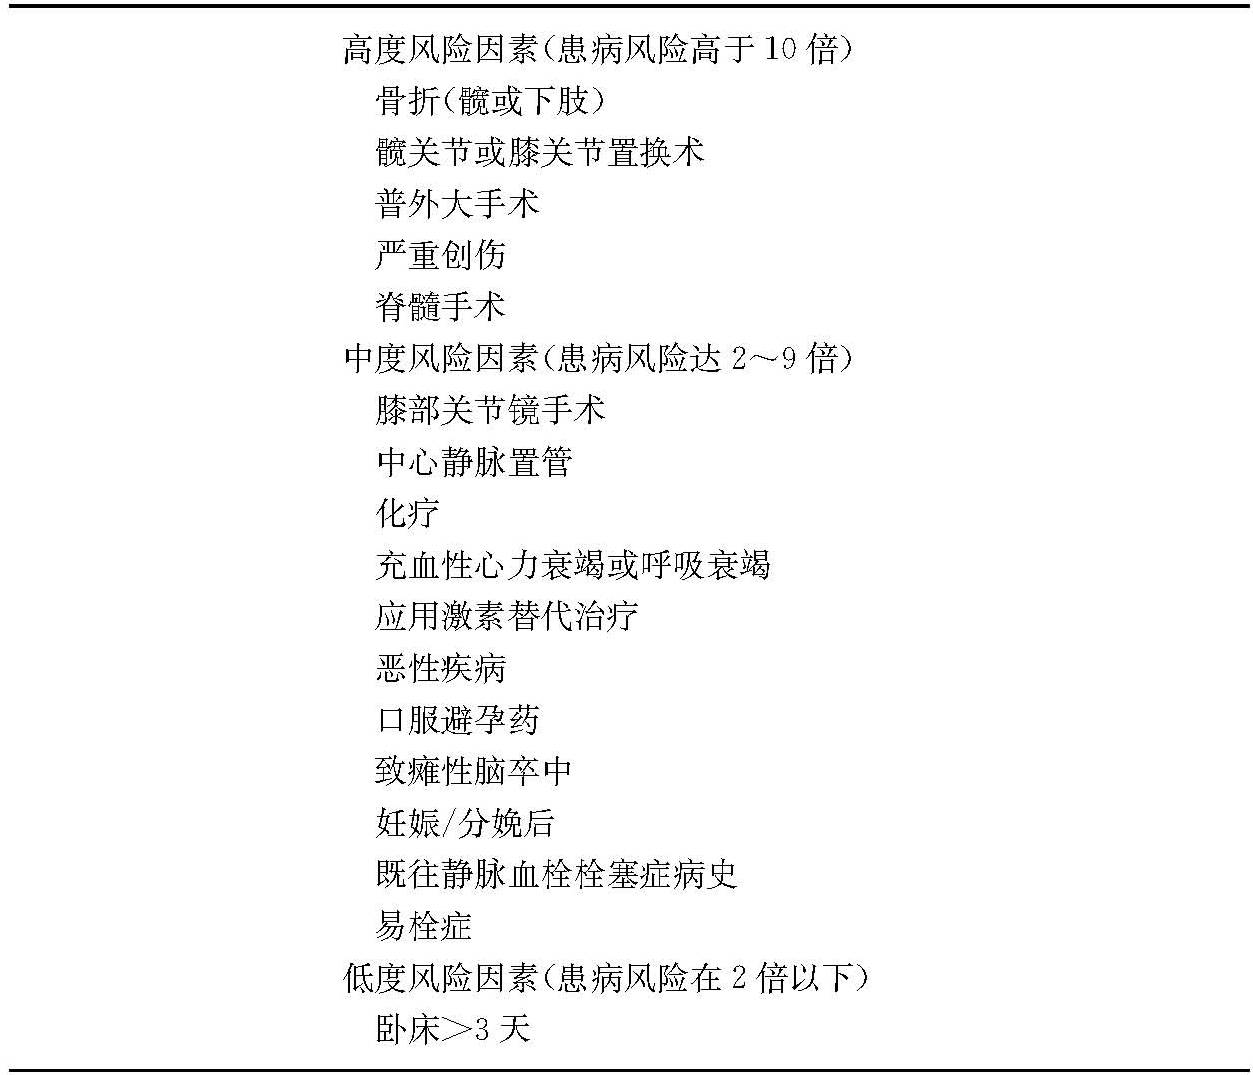
\includegraphics[width=\textwidth,height=\textheight,keepaspectratio]{./images/Image00119.jpg}
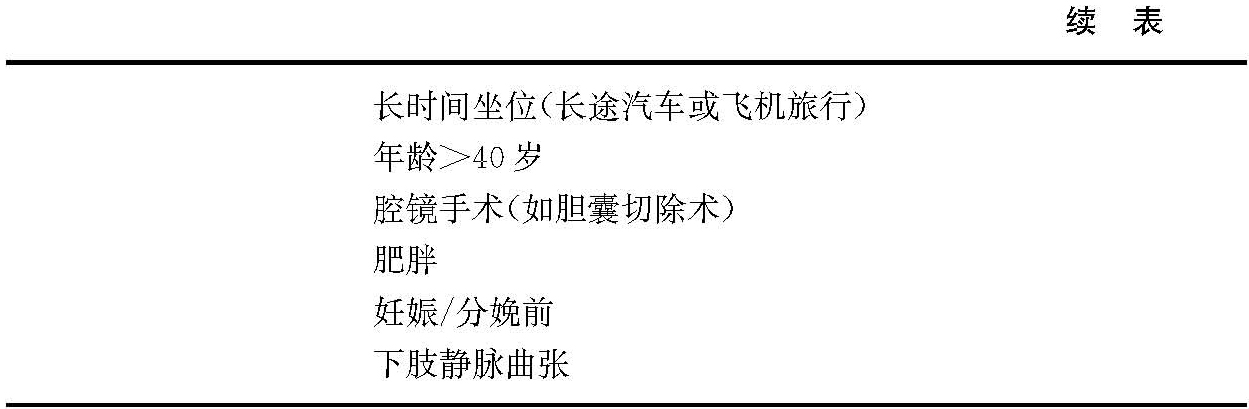
\includegraphics[width=\textwidth,height=\textheight,keepaspectratio]{./images/Image00120.jpg}
\end{table}

以上易患因素可单独或同时存在。在住院条件下,一般78%的患者暴露于静脉血栓栓塞症的易患因素之下,约20%的患者可能同时存在多个易患因素。住院患者中约18%~23%会发生静脉血栓栓塞症,易患因素越多,发生静脉血栓栓塞症的概率就越高。

\subsubsection{静脉血栓栓塞症的发病率是多少,我国静脉血栓栓塞症发病的现状如何?}

静脉血栓栓塞症患者中约2/3为单纯下肢深静脉血栓者,1/3合并肺血栓栓塞症。流行病学的资料显示,无论是普通人群还是住院患者,静脉血栓栓塞症的发病率都很高。普通人群中,男女年发病率分别为1.3‰和1.1‰。症状性下肢深静脉血栓发病率为145例/10万人,肺血栓栓塞症为69例/10万人。约1/3的静脉血栓栓塞症患者在10年内可能复发,高发期为首发后的6~12个月。目前已知美国每年确诊肺血栓栓塞症34万~60万例,死亡数约6万例/年,静脉血栓栓塞症的发病率排在心肌缺血综合征和脑卒中之后,居心血管疾病的第三位。

一项丹麦的4881例外科患者的调查中,尸检证实术后致死性肺血栓栓塞症的发生率为9%,接受静脉血栓栓塞症预防者和未接受者的病死率分别为3.5%和11.2%。在住院未接受抗凝的人群中,10%~26%发生静脉血栓栓塞症,骨科患者中静脉血栓栓塞症的发生率更是高达40%~60%。一个耐人寻味的现象是尽管外科患者更多地暴露于易患因素之下,75%的致死性肺血栓栓塞症却未发生于外科,尸检进一步证实非外科患者中约有7.6%的死亡由肺血栓栓塞症引起。

肺血栓栓塞症的发生率随着年龄的增长而增加,18岁以下青少年的发病率极低,约为(0~0.3)/10万人,且多集中于有基础疾病的人群中。40岁后每增加10岁静脉血栓栓塞症的发病率翻一番,发病高峰在70岁左右,75岁可达1%。性别方面,男性略高于女性,男女发病率之比为1.24∶1。在预后方面,下肢深静脉血栓的预后要好于肺血栓栓塞症,症状性肺血栓栓塞症早亡(early
death)的风险比静脉血栓栓塞症高18倍。

我国的流行病学资料至今十分有限。分析我国35家医疗单位75140例外周血管疾病患者的数据发现,深静脉炎和静脉曲张分别占11.6%和9.6%。上海市第九人民医院1990年在华东四省一市进行流行病学调查,发现下肢静脉疾病的发病率为8.72%,推测我国下肢深静脉血栓及存在后遗症的患者约有3000万例。中国医学科学院阜外心血管病医院连续900例尸检资料证实,肺段以上肺血栓栓塞症占心血管疾病的11.0%。242例住院肺血管病患者分类调查,肺血栓栓塞症占肺血管病的第一位。从近年来的文献报道来看,国内肺血栓栓塞症的发生率和检出率都呈指数级的增长,进一步说明肺血栓栓塞症并非少见疾病。

\subsubsection{症状性下肢深静脉血栓有何临床特点,为何要提倡预评分(pre-test)模式?}

多数下肢深静脉血栓患者可无自觉症状或临床表现,但由于可并发致死性肺血栓栓塞症和远期下肢深静脉功能障碍,危害极大,及时发现和治疗都有赖于对疾病的早期发现和正确诊断。下肢深静脉血栓的临床特征如下:

(1)多存在易患因素,如手术后、创伤、晚期肿瘤、昏迷或长期卧床的患者。

(2)起病较急,患肢肿胀、发硬、静脉走行区明显疼痛,活动后加重,偶有发热、心率加快。

(3)血栓部位压痛,沿血管走行区可扪及索状物,血栓远端肢体肿胀,皮肤呈青紫色或暗红色,皮温降低,足背、胫后动脉搏动减弱或消失,或出现静脉性坏疽。血栓延伸至下腔静脉时,双下肢、臀部、下腹和外生殖器均明显水肿。血栓发生在小腿肌肉静脉丛时,Homans征(直腿伸踝试验)和Neuhofs征(压迫腓肠肌试验)阳性。

(4)后期血栓机化,常遗留静脉功能障碍,出现浅静脉曲张、色素沉着、溃疡、肿胀等,称为下肢深静脉血栓后综合征(postthrombtic
syndrome)。

近年来静脉血栓栓塞症诊断方面非常提倡首诊的临床评分模式,也就是在相关实验室检查之前(pre-test),根据体检和病史进行评分,以此判断患者静脉血栓栓塞症的可能性。该方法结合随后进行的超声或D-二聚体检查可组合成不同的诊断策略,有效排查需要进一步检查与治疗的患者,提高诊断的成本效益比,非常适合门、急诊和住院患者使用。

目前已有的评分模式中,最常应用的就是Wells评分,已有至少14个研究证实Wells评分的可行性。Wells评分包括下肢深静脉血栓和肺血栓栓塞症两个评分,分别用于两者的临床诊断,下肢深静脉血栓评分参见表\ref{tab16-5}
\protect\hyperlink{text00022.htmlux5cux23ch8-21}{\textsuperscript{{[}8{]}}}
\textsuperscript{,}
\protect\hyperlink{text00022.htmlux5cux23ch9-21}{\textsuperscript{{[}9{]}}}
。如果评分≥2分,称为“疑似下肢深静脉血栓”,<2分者称为“非下肢深静脉血栓”。

\begin{table}[htbp]
\centering
\caption{下肢深静脉血栓临床评估模式表(Wells评分)}
\label{tab16-5}
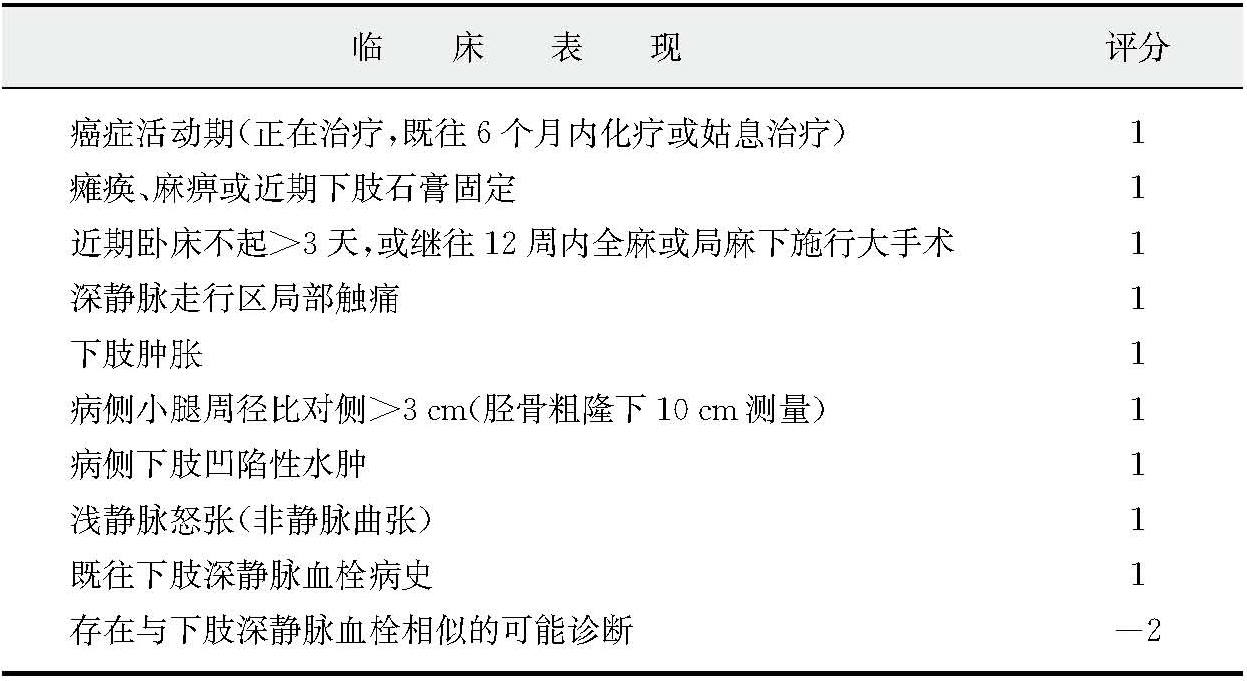
\includegraphics{./images/Image00121.jpg}
\end{table}

\subsubsection{肺血栓栓塞症临床症状与体征有何特点?}

肺血栓栓塞症临床症状与体征的特点可以归纳为:①表现谱广,极度缺乏特异性,从无症状到猝死差异很大,确诊依赖客观检查;②除原发病的表现外,肺血栓栓塞症患者多数呈合并症状,单独出现的症状体征较少见;③症状与疾病严重程度相关性不高,某些肺动脉主干栓塞的患者仅有轻微症状甚至无症状。

一般而言呼吸困难与气促是最常见的症状和体征
\protect\hyperlink{text00022.htmlux5cux23ch10-21}{\textsuperscript{{[}10{]}}}
,发生率84%左右,并尤以活动后明显。其他常见的症状依次为:胸膜样胸痛或心绞痛样疼痛、惊恐甚至濒死感、心动过速或心悸、晕厥、咳嗽、咯血。临床上出现所谓“PI三联征”(呼吸困难、胸痛及咯血)者不足30%。

体征方面除呼吸急促外,心动过速、肺部听诊啰音、肺动脉第二心音亢进、颈静脉怒张、血压变化、紫绀均较常见。肺血栓栓塞症患者的发热多为低热(<38℃),高热多发生于有并发症或大面积栓塞时。

与下肢深静脉血栓相同,近年来肺血栓栓塞症临床诊断方面最重要的进展就是强调临床决策规则(clinical
decision
rules,CDR)的重要性,并据此发展出多种预评分系统,这对于早期发现高度疑似的肺血栓栓塞症患者具有重要价值。目前最常用的临床决策规则评估系统就是Wells和Geneva两种肺血栓栓塞症临床评分表(表\ref{tab16-6}、表\ref{tab16-7})
\protect\hyperlink{text00022.htmlux5cux23ch9-21}{\textsuperscript{{[}9{]}}}
\textsuperscript{,}
\protect\hyperlink{text00022.htmlux5cux23ch10-21}{\textsuperscript{{[}10{]}}}
;Geneva评分与Wells评分类似,但需要血气分析和胸部X线的检查结果。其他亦在临床应用的评分还包括Miniati评分、Charlotte评分和修正Hyers评分。多项前瞻性研究已证实预评分的重要性,临床医师如能按照正式的规则在进一步进行相关检验或影像学检查前先行评估的话,后续诊治更有可能依循指南而行,反之,疑似肺血栓栓塞症患者则可能接受不适当的诊治,并影响预后。正因如此,目前的国际下肢深静脉血栓/肺血栓栓塞症指南中均已标明相应预评分标准。

\begin{table}[htbp]
\centering
\caption{Wells肺血栓栓塞临床评分表}
\label{tab16-6}

\includegraphics[width=\textwidth,height=\textheight,keepaspectratio]{./images/Image00122.jpg}
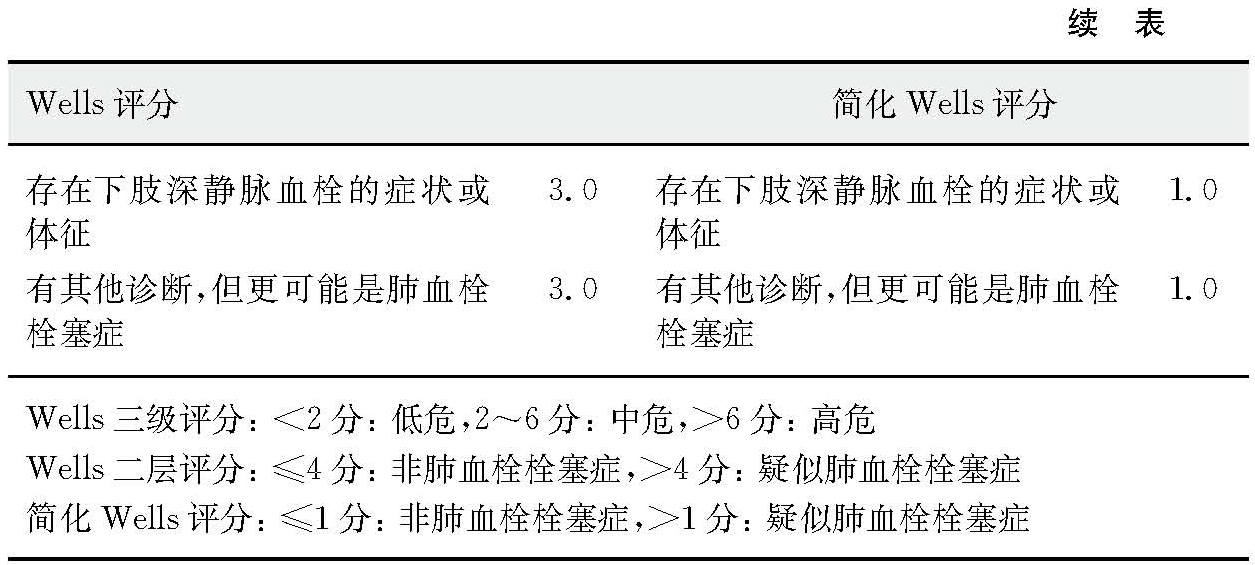
\includegraphics[width=\textwidth,height=\textheight,keepaspectratio]{./images/Image00123.jpg}
\end{table}

\begin{table}[htbp]
\centering
\caption{Geneva系列肺血栓栓塞临床评分表}
\label{tab16-7}
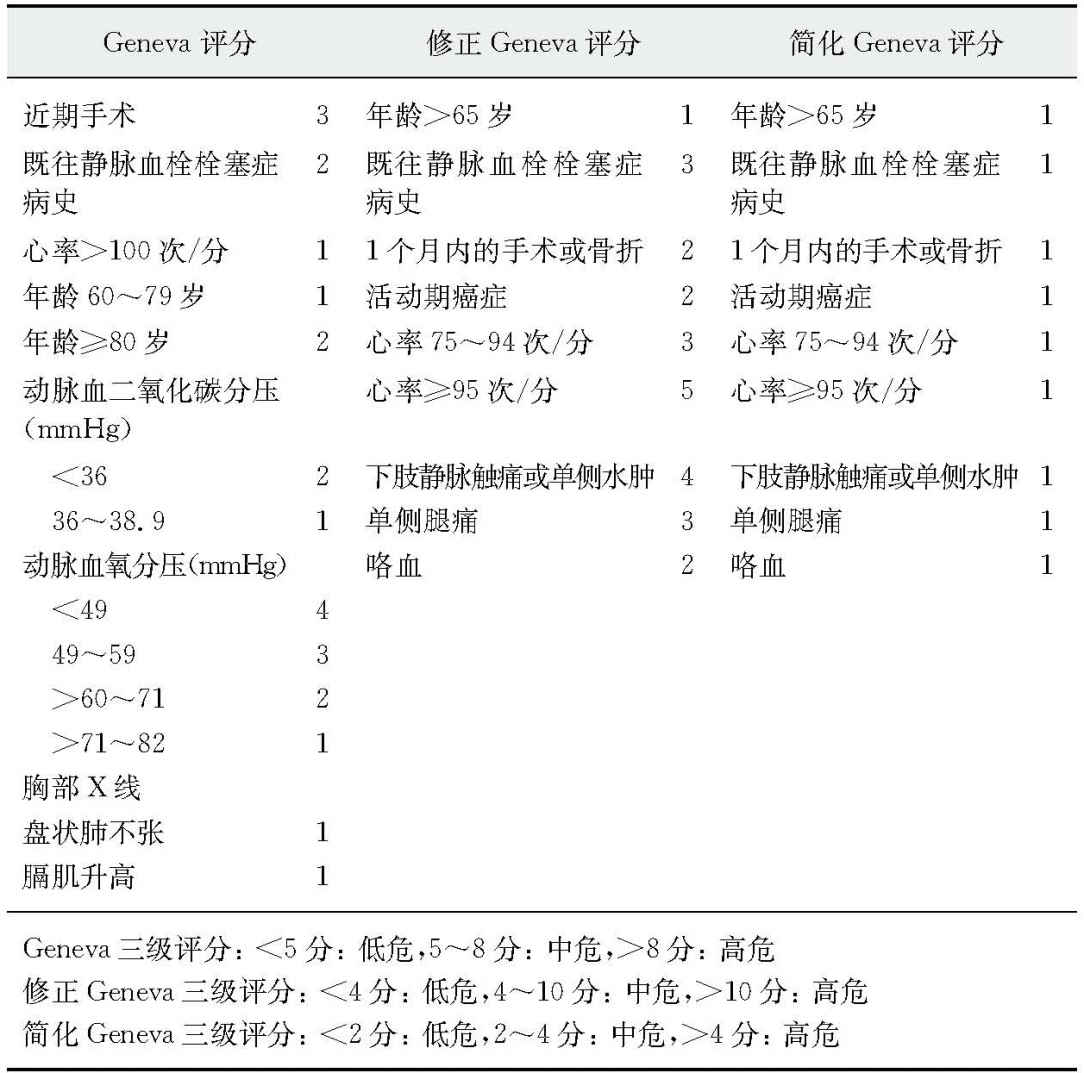
\includegraphics[width=\textwidth,height=\textheight,keepaspectratio]{./images/Image00124.jpg}
\end{table}

\subsection{辅助检查部分}

\subsubsection{下肢深静脉血栓的辅助检查有哪些,应用价值如何?}

可根据患者病情、医院设备、医生经验等做如下选择。

(1)加压超声成像(compression
ultrasonography) 为无创检查,现已成为筛查的首选手段。通过探头压迫观察等技术,可发现85%以上的近端下肢静脉血栓,静脉不能被压陷或静脉腔内无血流信号为下肢深静脉血栓的特定征象和诊断依据。其对股静脉血栓的敏感性达97%,特异性98%。但对腓静脉及其以下血栓或无症状的下肢深静脉血栓敏感性仅73%。

既往认为,对于临床高度可疑者,如加压超声成像阴性应于5~7天后复查。但近年来该说法受到质疑,因研究发现,仅1%~2%的患者在复查时发现有近端下肢深静脉血栓,因此成本效益比并不理想。

(2)血浆D-二聚体的测定 用酶联免疫吸附试验检测,敏感性高达95%~100%,其阴性似然比(negativelikehoodratio)为0.1。因此D-二聚体阴性的价值远远高于阳性的价值,用于排除诊断更有意义。急性下肢深静脉血栓或肺血栓栓塞症时,D-二聚体多>500μg/L,故常以D-二聚体<500μg/L作为排除诊断的阈值。临床评分模式“低可能性”+D-二聚体阴性,随访3个月静脉血栓栓塞症的发生率仅为0.4%~0.5%,因此这部分患者不必再行加压超声成像检查和抗凝治疗,预后也是安全的。

(3)放射性核素血管扫描检查(radionuclide
venography) 利用核素在下肢深静脉血流或血块中浓度增加,通过扫描而显像,是对下肢深静脉血栓诊断有价值的无创检查。诊断的准确性达80%~90%,敏感性在90%以上,并适用于对造影剂过敏者。

(4)SCT静脉造影(computed
tomo-venography) 螺旋CT血管造影技术近年来发展很快,其优点是成像迅速,可在肺血管造影完成后2~3分钟内完成下肢静脉横断扫描,同时获得肺血栓栓塞症及下肢深静脉血栓的情况。在进行CT肺血管造影的同时不需另外添加造影剂,使下肢静脉、盆腔静脉及下腔静脉迅速显影,因此近年来应用广泛。

(5)静脉造影(venography) 是确定诊断的“金标准”,可显示静脉堵塞的部位、范围、程度及侧支循环和静脉功能状态,其诊断敏感性和特异性接近100%。但其有创性限制了临床推广应用。

(6)阻抗体积描记测定 其原理是在大腿处放置一个袖带,探测充气前后下肢血流量的变化,袖带放气,下肢容量迅速恢复到基线水平被用作是静脉可变性指数。阻抗体积描记测定对无症状下肢深静脉血栓的敏感性差,对有症状的近端下肢深静脉血栓具有很高的敏感性和特异性,且操作简单,费用较低。

(7)磁共振静脉造影 为无创性检查,可同时显示双下肢静脉,并能准确地确定盆腔和下腔静脉的血栓,有潜在的鉴别急、慢性血栓的功能。对有症状的急性下肢深静脉血栓诊断的敏感性和特异性可达90%~100%。磁共振静脉造影在检出盆腔和上肢深静脉血栓方面有优势,对无症状的下肢深静脉血栓具有很好的临床应用前景。

通过不同的检查步骤和检查仪器可制定相应的诊断策略或诊断流程,任何诊断策略的建立都应在兼顾患者利益的前提下,以高成本效益比为原则。下肢深静脉血栓的诊断策略参见图\ref{fig16-1}:基于临床所见和病史首先进行预评分,初步判断患者下肢深静脉血栓的可能性,然后结合D-二聚体结果与下肢超声的组合策略完成诊断并给予治疗。需要强调的是,诊断下肢深静脉血栓时,应同时考虑有无肺血栓栓塞症存在,反之亦然。

\begin{figure}[!htbp]
 \centering
 
\includegraphics{./images/Image00125.jpg}
 \captionsetup{justification=centering}
 \caption{下肢深静脉血栓诊断步骤}
 \label{fig16-1}
  \end{figure} 

\subsubsection{肺血栓栓塞症的辅助检查有哪些,有何进展?}

肺血栓栓塞症的诊断主要依靠客观的辅助检查,包括动脉血气、心电图、X线胸片、超声心动图、下肢静脉血栓检查、D-二聚体、肺通气/灌注显像、肺动脉造影和螺旋CT、MRI静脉造影等检查,一方面明确肺血栓栓塞症的临床诊断,另一方面在于明确肺血栓栓塞症常见病因下肢深静脉血栓的诊断。现将近年来的各项检查的进展分述如下。

(1)常规检查 大多数肺血栓栓塞症患者血气分析会出现低氧、低碳酸血症和肺泡动脉血氧分压差增大。通常低氧血症的程度与栓塞的程度相关,但有12%~23%既往无心肺疾病的患者动脉血氧分压在80~100mmHg之间,如单纯以血气分析作为肺血栓栓塞症的筛选指标会造成诊断假阴性。低氧血症和肺泡动脉氧分压差改善的程度与肺灌注缺失的恢复相关。

肺血栓栓塞症患者心电图常表现为窦性心动过速或者未见明显异常,右心负荷严重增加时可表现为S\textsubscript{Ⅰ}
Q\textsubscript{Ⅲ} T\textsubscript{Ⅲ}
形式,心电轴右偏,V\textsubscript{1} 、V\textsubscript{2}
导联ST段下移,T波改变,甚至出现完全性右束支传导阻滞。T波倒置有助于确定病变程度,特别对于大面积栓塞,其特异性为68%。以上心电图的异常表现也预示患者预后不良,多元回归分析证实上述任何一种心电图变化都是不良预后的独立易患因素。

40%的肺血栓栓塞症患者X线胸片常无明显异常,异常表现亦多为非特异性的,与心电图相似,其更多用于排除诊断。X线胸片常见的特征是:肺动脉增宽,区域性肺血管纹理稀疏、纤细、肺野透亮度增加,膈肌抬高,肺动脉搏动增强,心影扩大和胸膜渗出,肺梗死时出现特征性的楔形阴影。X线胸片的敏感性和特异性虽不高,但它不失为一种简便快速的诊查手段。必须强调的是,所有疑似肺血栓栓塞症的患者都应该常规进行心电图和X线胸片检查。

(2)生物标志物检查

D-二聚体 D-二聚体是纤溶过程中交联纤维蛋白的降解产物,当出现血栓活化时,D-二聚体常高于正常,因此具有极高的敏感性,适合于术前或急诊下肢深静脉血栓高危患者的筛查。

D-二聚体极易受基础疾患如外伤、妊娠、恶性肿瘤、全身性感染等的干扰,术后患者D-二聚体几乎都呈阳性,因此对于下肢深静脉血栓的诊断或者鉴别诊断价值不大。80岁以上的高龄患者特异性较低,不宜使用。

目前主要有5种测定D-二聚体的方法:①酶联免疫吸附试验的敏感性最高,达98%,但特异性仅45%,此法价格较贵且费时;②快速酶联免疫吸附测定法敏感性和特异性分别为94%和50%,优点是用时短;③全血红细胞凝集试验,如商品化的SimpliRED,敏感性和特异性分别为85%和70%,测定快速,且可在床边测定;④浊度计法,敏感性达95%以上,测定时间约为两小时;该方法是胶乳凝集试验,其成本低廉,但敏感度过低,不足以用于排除静脉血栓栓塞症,因此对静脉血栓栓塞症的诊断帮助不大;⑤基于免疫比浊法的乳胶凝集试验(如Microlatex法)可用于定量分析血浆的D-二聚体浓度。一项多中心研究比较了酶联免疫吸附试验法与Microlatex法在门诊和病房测定D二聚体,发现两种方法对于门诊患者的敏感性与特异性均高于病房患者(表\ref{tab16-8})。

\begin{table}[htbp]
\centering
\caption{门诊与病房两种D-二聚体测定方法的比较}
\label{tab16-8}
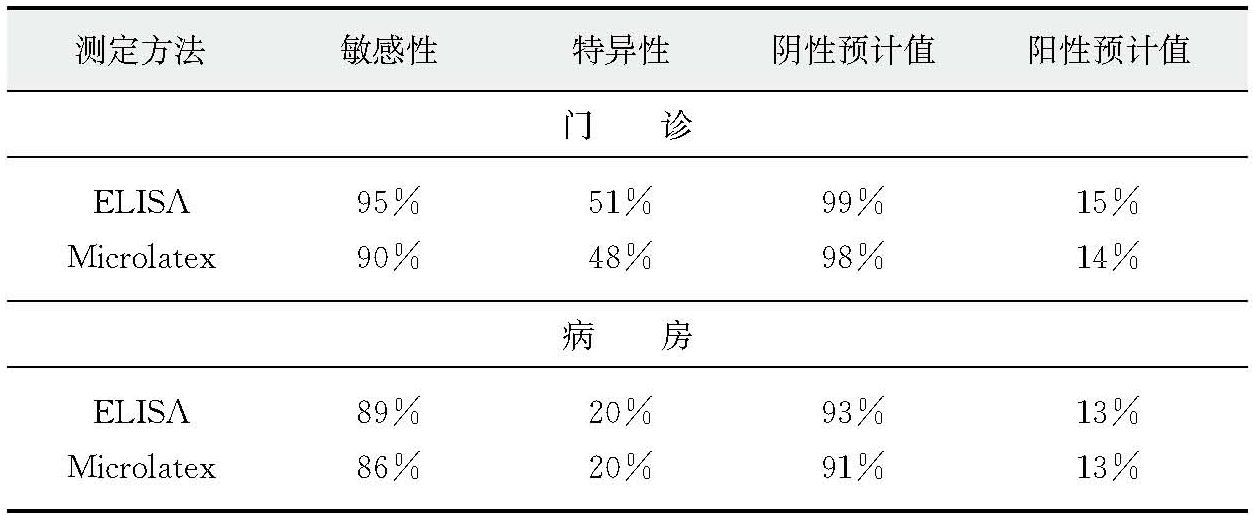
\includegraphics{./images/Image00126.jpg}
\end{table}

大量研究证实,临床评分结合D-二聚体能够大大提高后者在排除静脉血栓栓塞症诊断方面的价值。930例的大样本研究发现,SimpliRED法结合临床评估,D-二聚体的阴性预计值达到99.5%。D-二聚体还可作为监测静脉血栓栓塞症是否复发的工具。研究发现,接受治疗的静脉血栓栓塞症患者在随访期间应用酶联免疫吸附试验法测定D-二聚体<250μg/L者,2年静脉血栓栓塞症的复发率仅为3.7%,而高于250μg/L者为11.5%。但目前的证据还没有发现D-二聚体与国际标准化比值具有相关性,因此不能用国际标准比值作为判断抗凝疗效的指标。

心肌肌钙蛋白I和T 心肌肌钙蛋白测定近年来逐渐成为评估肺血栓栓塞症预后的热点。作为心肌损伤的特异性标志物,肺血栓栓塞症患者心肌肌钙蛋白I和心肌肌钙蛋白T的升高意味着右室扩张、微小梗死灶形成和心肌损伤,并与病情程度和预后密切相关。心肌肌钙蛋白T阈值为0.09μg/L时,预测院内病死率敏感性为80%、特异性为92%、阴性预测值99%、阳性预测值为34%。另一项回归分析也同样发现,心肌肌钙蛋白I升高组死亡的风险是对照组的17倍。

近期的“肺血栓栓塞治疗策略与预后研究-2”就心肌肌钙蛋白I、心肌肌钙蛋白T在评价肺血栓栓塞症预后和危险分级方面进行了探讨
\protect\hyperlink{text00022.htmlux5cux23ch11-21}{\textsuperscript{{[}11{]}}}
。106例肺血栓栓塞症患者中心肌肌钙蛋白I阳性者(≥0.07μg/L)为41%,心肌肌钙蛋白T阳性者(0.04μg/L)为39%,98%的患者心肌肌钙蛋白I和心肌肌钙蛋白T在疑诊肺血栓栓塞症的4小时内开始升高,超声心动图可见右室功能障碍,且不良预后与其阳性明显相关,心肌肌钙蛋白I和心肌肌钙蛋白T阴性预计值分别为92%和93%,但由于两者在非肺血栓栓塞症患者中亦有升高,因此其阳性预计值分别为37%和41%。

脑钠肽 脑钠肽是心房利钠肽家族的成员之一,主要由于心房受牵张后分泌增加,既往多用于慢性心力衰竭和急性冠脉综合征的诊断及预后判断。目前已有该指标用于肺血栓栓塞症的报道。73例患者以脑钠肽前体500ng/L为阈值分为两组。结果发现,脑钠钛前体>500ng/L组的症状、血液动力学和右室功能障碍均比脑钠钛前体<500ng/L组严重。以脑钠钛前体500ng/L为阈值,判断肺血栓栓塞症患者不良预后的敏感性为95%,特异性为57%,阴性预计值97%,阳性预计值45%
\protect\hyperlink{text00022.htmlux5cux23ch12-21}{\textsuperscript{{[}12{]}}}
。

心肌肌钙蛋白和脑钠肽等心脏特异性标志物对急性肺血栓栓塞症的诊断价值在于发现右心室过度牵张、右室功能障碍的高危肺血栓栓塞症患者,此类患者是否应该给予溶栓是目前肺血栓栓塞症治疗领域的争议所在,较为保守的观点认为该治疗方案目前尚无确切的证据支持,还有待相关的研究和共识性策略出台。

(3)通气/血流扫描

通气/血流扫描曾是肺血栓栓塞症最为常用的无创性筛查手段,对治疗以及随访均极具价值。根据通气与灌注是否匹配将结果分为3类:①高度可能,征象为至少一个或更多叶段的局部灌注缺损而该部位通气良好或X线胸片无异常;②正常或接近正常;③非诊断性异常,其征象介于高度可能与正常之间。一般认为灌注显像正常与肺动脉造影正常具有同等的诊断价值;显像正常的疑似患者不进行抗凝治疗没有严重后果。但目前认为通气/血流扫描在肺血栓栓塞症诊断中的作用很有限。1990年美国的肺血栓栓塞诊断的前瞻性调查(PIOPED)研究
\protect\hyperlink{text00022.htmlux5cux23ch13-21}{\textsuperscript{{[}13{]}}}
发现,若临床评价与显像结果相符,通气/血流扫描确定或排除肺栓塞的准确率很高。例如临床高可能性+通气/血流扫描高度可疑者,诊断率达96%。如两者均为低度可疑,则仅有4%的患者为肺血栓栓塞症。但实际上临床评价与显像结果相符的患者仅占患者总数的1/3,约2/3的疑似肺血栓栓塞症患者的确诊依然要靠肺动脉造影。除此之外,通气/血流扫描对肺水肿、右心衰、低血压等心肺储备功能低的患者的应用价值不大,其检查程序和费用也不具备明显的优势,因此临床通气/血流扫描的应用已逐步减少,逐步被更为敏感和快速的CT肺血管造影或MRI动脉造影所代替。

近期,通气/血流扫描的研究进展是应用新型的核素血栓显像剂------\textsuperscript{99m}
Tc标记的抗人活化血小板单克隆抗体,有助于鉴别新鲜血栓或陈旧血栓,这有助于提高急性肺血栓栓塞症的诊断率。此外,应用核素标记的特异性D-二聚体抗体,通过单光子发射体层成像技术诊断肺血栓栓塞症和下肢深静脉血栓在动物实验中也已有报道
\protect\hyperlink{text00022.htmlux5cux23ch14-21}{\textsuperscript{{[}14{]}}}
,很有可能成为未来核医学诊断肺血栓栓塞症的方向。

(4)肺动脉造影 尽管肺栓塞的诊查手段进展迅猛,肺动脉造影仍旧是肺栓塞诊断的“金标准”。其敏感性约为98%,特异性为95%~98%。肺血栓栓塞症的直接征象有肺血管内造影剂充盈缺损,伴或不伴轨道征的血流阻断;间接征象有肺动脉造影剂流动缓慢,局部低灌注,静脉回流延迟等。其潜在的应用优势在于除了能够通过导管直接诊断外,在有条件的医院还可以同时进行下腔静脉滤器植入及局部介入取栓或溶栓。

肺动脉造影作为有创性检查,其应用受到限制。根据PIOPED对1111例肺动脉造影的报告,肺动脉造影的准确率为96%,3%无诊断意义,0.4%为假阴性。检查过程中5例(0.45%)死亡,9例(0.81%)发生肾衰、呼吸窘迫、血管损伤、造影剂过敏等较严重的并发症,并以有严重基础疾病的患者多见。由于慢性血栓机化与血管壁融合使造影的对比效果不佳,肺动脉造影对慢性肺动脉高压的陈旧性血栓敏感性差。另一个要考虑的问题是放射科医师阅片的一致性,一般对肺动脉主干栓子的诊断一致性为98%,而亚段血栓仅为66%。

总之,肺动脉造影尽管确诊意义最大,但在临床中的应用并不广泛,多用于其他诊察手段无肯定性结论的高度疑似患者。

(5)螺旋CT、高分辨率CT与CT肺血管造影

CT肺血管造影诊断肺血栓栓塞症的直接征象为造影剂的充盈缺损、完全梗死及轨道征;间接征象为肺总动脉、左或右肺动脉扩张,血管断面细小、截断、肺梗死灶等。单层或多层CT肺血管造影为肺血栓栓塞症的诊断提供了无创性的选择,具有直接显示肺血管、扫描速度快、分辨率高和无影像重叠等多种优势,对肺段以上的栓塞有着良好的显示效果,目前已经替代肺动脉造影而成为肺血栓栓塞症的一线检查手段,其应用前景十分看好,单独或与其他诊断方法结合应用,对肺血栓栓塞症的诊断均有很高的临床价值。对螺旋CT的异议在于其不能可靠地显示亚段水平的血栓,敏感性仅为63%;其次,螺旋CT不能提供血液动力学资料。

螺旋CT的技术进展 近年来多层螺旋CT得到广泛应用,大大缩短了扫描时间,可在一次屏气下行1mm层厚的全肺薄层扫描,对周围肺动脉的观察能力明显增强,提高了肺动脉造影的诊断准确率。2006年《New
England Journal Medicine》刊登了PIOPEDⅡ的研究报告
\protect\hyperlink{text00022.htmlux5cux23ch15-21}{\textsuperscript{{[}15{]}}}
。通过多层CT肺血管造影结合CT静脉造影(CT肺血管造影CT静脉造影)诊断急性肺血栓栓塞症,结果发现,CT肺血管造影敏感性为83%,特异性为96%,结合临床高/低度可能性,相应的阳性预计值达96%,中度临床可疑者则为92%。如果临床可能性评价与CT肺血管造影不符,则无诊断意义。CT肺血管造影---静脉CT造影诊断急性肺血栓栓塞症的敏感性为90%,特异性为95%,若临床可能性评价与CT肺血管造影---静脉CT造影不符,则无诊断意义,故而CT肺血管造影静脉CT造影较单独的CT肺血管造影有更高的诊断敏感性;与临床评估综合应用时,若其可疑度与临床评估相同,则诊断预计值较高,反之可能需要其他的辅助检查。

随着多层螺旋CT的技术进步,目前“CT心脏测量(cardiac CT
measurements”)已成为可能,并逐渐成为肺血栓栓塞症影像诊断的热点。研究发现,右心室短轴(RV
short axis)或右/左心室直径之比(RV/LV diameter
ratio)可作为判断肺血栓栓塞症不良预后的指标,在CT四腔室影像中,右/左心室直径比值>1者诊断右室功能障碍的敏感性为78%,特异性100%,阳性预计值100%;“右心室增大”预计30天病死率的敏感性、特异性、阴性预计值与阳性预计值分别为78.2%、38%、15.6%和92.3%。其他的方法还有测量下腔静脉/奇静脉或腔室面积,后者更为精确。也有学者报道肺动脉直径测量、肺动脉栓子负荷指数(pulmonary
artery clot load
scores)、室间隔左移、下腔静脉造影剂反流等指标,但尚存在争议。

近期,CT肺血管造影检查产生的辐射暴露已成为热点话题。单次CT肺血管造影的照射剂量为3~5mSV,相当于接受1~2年的日常背景辐射。根据年龄与性别的不同,此暴露剂量相当于导致(38~180)例/10万肺癌的发生;尤其对年轻妇女而言辐射对乳腺组织的影响不能忽视,该剂量可使乳腺癌的发生率高达503/10万。为此,美国放射学协会推荐初诊影像学医师及育龄期妇女要谨慎进行CT肺血管造影检查。

未来螺旋CT的研究方向将包括:动态肺动脉造影结合加权色彩编码实现肺部大循环和微循环的灌注显像;通过多层螺旋CT结合心电图门控技术实现右心功能的动态评价,例如射血分数和右室室壁运动异常。如果以上技术继续发展下去,未来就可能出现螺旋CT替代目前已有的超声心动图、肺动脉造影,通过单次螺旋CT检查完成诊断和预后风险评估的局面,这无疑将大大优化诊断的成本---效益比。

螺旋CT的诊断敏感性与特异性荟萃分析显示,CT肺血管造影诊断肺血栓栓塞症存在明显的异质性,肺血栓栓塞症的检出率为19%~79%,敏感性为88.9%[95%可信区间(CI)82.0%~95.0%],特异性为94.6%(95%CI91.3%~98.0%),对外周血栓特异性仅79%。假阴性率1.0%~10.7%,若CT肺动脉造影和下肢深静脉血栓检查均为阴性,则假阴性率为1.5%(95%CI1.0%~1.9%);若CT肺动脉造影和下肢深静脉血栓检查均为阴性者,随访发现预后良好,不必抗凝治疗
\protect\hyperlink{text00022.htmlux5cux23ch16-21}{\textsuperscript{{[}16{]}}}
。

2005年《JAMA》的荟萃分析报道,CT肺动脉造影阴性结果的阴性预计值达到99.1%,单层螺旋CT阴性结果静脉血栓栓塞症的阴性似然比为0.08,多层螺旋CT为0.15,CT肺动脉造影阴性结果对于肺血栓栓塞症死亡的阴性似然比为0.01,阴性预计值为99.4%,可见CT肺动脉造影阴性患者的预后良好,与标准肺动脉造影并无差别
\protect\hyperlink{text00022.htmlux5cux23ch17-21}{\textsuperscript{{[}17{]}}}
。

与其他诊断手段的比较 早期报道发现,CT肺动脉造影与通气/血流扫描比较,当扫描结果为高度可疑时,螺旋CT的敏感性和特异性分别为87%和95%,通气/血流扫描的敏感性和特异性分别为65%、94%。荟萃分析显示:螺旋CT的整体敏感性为86%,特异性93.7%。通气/血流扫描对临床高度可疑者的敏感性为39%,特异性97.1%;对于非可疑者的敏感性为98.3%,而特异性仅4.8%。结论是CT肺动脉造影在排除肺血栓栓塞症方面明显优于通气/血流扫描,但对于高度疑似的患者两者的诊断效力相似。

(6)MRI MRI及MRI肺动脉造影已开始用于临床研究。早期的研究由于受呼吸的影响,及血流与栓子的对比效果不佳而欠理想。目前通过应用镓增强已能够在单次呼吸时得到高分辨率的影像。与标准肺动脉造影和MRI动脉造影比较,MRI的敏感性90%,特异性77%,阳性预计值86%,阴性预计值83%。但对亚段栓子敏感性不佳,不能可靠地显示出直径<4mm的外周栓子,且阅片者间有较大的差异。MRI的缺点还包括扫描时间长,肺动、静脉同时显影,呼吸和心动伪影使诊断受到限制。MRI的优势在于可准确、清晰地分辨急性和慢性下肢深静脉血栓,并对外周深静脉血栓很敏感,可很好地区分下腔静脉和骨盆静脉,避免标准肺动脉造影中造影剂对肾的损害。与螺旋CT相比,其对慢性栓塞的诊断效果是一样的;但对急性栓塞,螺旋CT的准确性要优于MRI。通气/血流扫描及临床评价同为高度可疑时,以肺动脉造影为标准,MRI和螺旋CT敏感性分别是71%、73%,特异性同为97%。但由于MRI价格昂贵,相关的对照研究受到限制,使其临床应用无法像螺旋CT那样普及,目前多用于造影剂过敏或潜在肾功能障碍的疑似肺血栓栓塞症的筛查。

2010年发表的PIOPED
Ⅲ评价了增强MRI肺动脉造影联合静脉造影对肺血栓栓塞症的诊断价值,初步结果显示,与CT肺动脉造影相比,MRI肺动脉造影可获得相同质量的影像学资料:MRI肺动脉造影诊断肺血栓栓塞症的敏感性为78%,特异性为99%;如联合MRI静脉造影,则其诊断敏感性可提高到92%
\protect\hyperlink{text00022.htmlux5cux23ch18-21}{\textsuperscript{{[}18{]}}}
。MRI肺动脉造影有其优越之处,可降低因射线辐射或造影剂注射引起风险,可获得肺通气血流分布资料,并可有效评价右心功能。但与CT相比,MRI肺动脉造影检查更复杂,技术要求高且稳定性差,在PIOPED
Ⅲ中,MRI肺动脉造影扫描图像不佳者占25%,MRI肺动脉造影联合MRI静脉造影影像技术不合格者占52%,这些患者由此无法得到明确诊断。另外,由于MRI肺动脉造影的检查时间长,重症患者难以接受此项检查。由于上述限制,目前MRI肺动脉造影仅推荐用于有经验的中心作为二线检查方法。

(7)超声心动图 超声心动图对近端栓子诊断的敏感性很高,同时又有助于鉴别与肺血栓栓塞症相似的疾病,如心肌梗死、心包炎等。肺栓塞时超声心动图的主要征象包括右心室扩张、右/左心室直径比值增加、近端肺动脉扩张、三尖瓣反流、右室流出道湍流、下腔静脉增宽等。如超声心动图发现右心负荷过重、室壁运动减弱以及肺动脉高压的征象,高度怀疑肺栓塞。就目前而言,超声心动图及多普勒检查对于病情和疗效的判断非常有价值。

近年来的进展是经食管超声心动图的应用。研究表明,经食管超声心动图检查优于经胸超声,其诊断敏感性为80.5%,特异性为97.2%;而经胸超声的敏感性为56%,特异性为90%。经食管超声心动图检查多用于肺总动脉或右肺动脉栓子的探查,能较好地显示较大的栓子。经食管超声心动图检查的优势还在于其快速、简便、可在床旁检测,可迅速对患者做出诊断,且可指导溶栓治疗。经食管超声心动图检查的缺点在于它是一种半有创性检查,不适合危重患者,且依赖于操作者的技术,对远端较小的栓子敏感性差。

超声诊断肺血栓栓塞症最常用于右室功能障碍,用以筛查可能需要溶栓的高危患者。研究发现,血压正常但超声心动图出现右室功能障碍的患者病死率达9.3%,而对照组仅为0.4%。多数研究以量化的右室运动度减低评价右室功能障碍,但荟萃分析发现目前并无“右室功能障碍”确切统一的超声诊断标准,这造成了研究结论的异质性,也使确认右室功能障碍需要溶栓的说法陷入尴尬的境地。

Kasper认为,右室扩张或右心室舒张末期直径>30mm,或者符合以下两项者可以考虑诊断右室功能障碍:①三尖瓣反流速度>2.8m/秒;②三尖瓣反流速度>2.5m/秒且不伴下腔静脉吸气相塌陷;③右肺动脉扩张(>12mm/m\textsuperscript{2}
);④右室室壁增厚>5mm,⑤下腔静脉吸气相塌陷。而Grifoni诊断右室功能障碍的标准包括:右室扩张(右室舒张末期直径>30mm或舒张末期右/左心室直径比值>1);矛盾性室间隔运动或肺动脉高压,且必须排除右室壁增厚(壁厚>7mm)。

(8)亚段栓子的临床意义 通气/血流扫描、CT肺动脉造影、MRI或经食管超声心动图检查等技术对近端栓子的诊断敏感性相差不大,但对亚段或亚段以下水平的栓子敏感性均较差。过去认为的“金标准”------肺动脉造影在亚段水平的诊断一致性也仅为66%。有研究表明,肺动脉造影对亚段水平的肺栓塞敏感度仅为87%,阳性预计值88%,与螺旋CT几乎无显著性差异,这就引出一个重要的问题:亚段血栓的临床意义是什么?

亚段肺血栓栓塞(subsegmental pulmonary
embolism)是指位于肺动脉第4级分支,相当于肺段动脉与小叶前动脉之间、直径为1~6mm的血栓栓塞,可能还包括更外周的或肺段动脉内的微小血栓。一般情况下,栓子会分裂为6~8个碎片,其中至少会有1块或更多的碎片大到足以被肺动脉造影或螺旋CT发现。单纯的亚段肺血栓栓塞可能并不常见,与典型肺血栓栓塞症相比,也无特异性的临床表现,甚至可能无症状;广泛的亚段肺血栓栓塞还可能造成慢性血栓栓塞性肺动脉高压。目前亚段肺血栓栓塞的诊断主要依赖于客观的辅助检查,尤其是肺动脉造影。已有的资料对亚段肺血栓栓塞的检出率报道差异较大,为6%~30%。栓塞部位以右肺和下叶多见,其中下叶各基底段为最好发部位。

部分学者认为亚段血栓多来源于腓部以下的深静脉微小血栓,对机体的影响不大,不必抗凝治疗。PIOPED研究发现,尽管亚段肺血栓栓塞可能会漏诊漏治,但通过1年随访,所有未经治疗的造影阴性者中仅有0.6%出现肺血栓栓塞症症状。对螺旋CT的荟萃分析也发现,螺旋CT阴性的疑似肺血栓栓塞症患者经过3个月随访,静脉血栓栓塞症的发生率仅1.4%,此结果支持亚段血栓栓塞无重要临床意义的推论。但相反的意见则认为亚段血栓的存在至少会提示以下问题:是否是下肢深静脉血栓或肺内出现大栓子的先兆;对于心肺储备功能低下的患者,微小栓子也可造成显著的血液动力学改变,有可能成为潜在的致死性诱因,或因反复无症状性的栓塞而导致慢性血栓栓塞性肺动脉高压,因此仔细探查和治疗亚段血栓十分重要。尽管目前多数研究支持亚段栓子意义不大的结论,但是个体化的判断与治疗还是必要的。

(9)肺血栓栓塞症的诊断策略 肺血栓栓塞症的生前误诊率高达70%,其原因与临床医生重视程度不足、肺血栓栓塞症的临床表现无特异性、缺乏敏感的诊断手段或诊断策略有关。许多医生试图结合多种诊察手段,以减少患者负担、提高诊断准确率和诊断成本---效益比,其原则包括评估前述的Wells标准,根据静脉血栓栓塞症的可能性大小在之后的诊断流程中尽早采用D-二聚体结合高敏感性的影像技术(图\ref{fig16-2})。后者如果为阴性,则不需进一步检查和治疗,因为已有大样本研究发现此类患者出现致死性的肺血栓栓塞症的风险极小。也有研究者考察了15种包括通气/血流扫描、下肢超声、螺旋CT、肺动脉造影和D-二聚体等方法的肺血栓栓塞症诊查策略,发现CT
肺动脉造影可以节省成本并增强效果,提示螺旋CT在今后诊断中的重要地位。

\begin{figure}[!htbp]
 \centering
 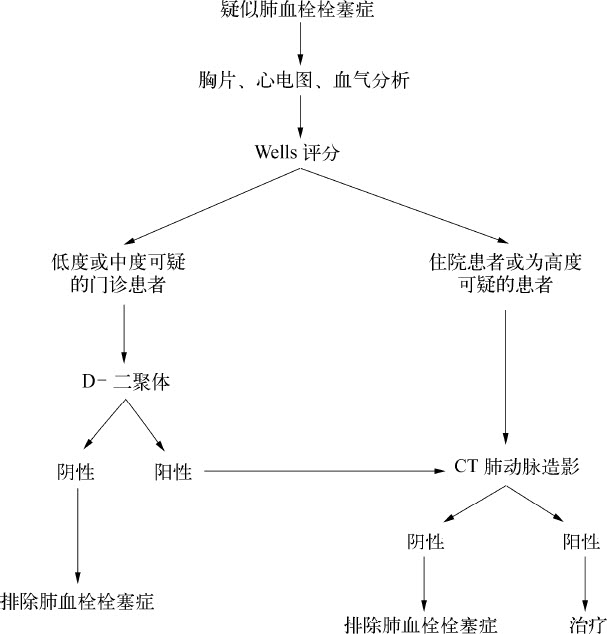
\includegraphics{./images/Image00127.jpg}
 \captionsetup{justification=centering}
 \caption{肺血栓栓塞症的诊断步骤}
 \label{fig16-2}
  \end{figure} 

研究发现,通过临床评估,D-二聚体和螺旋CT组成的诊断策略具有良好的可操作性,D-二聚体阴性者3个月随访出现非致死性静脉血栓栓塞症约0.5%,CT肺动脉造影阴性者3个月随访静脉血栓栓塞症的发生率为1.3%,有7例(0.5%)患者的死因可能是肺血栓栓塞症。

\subsection{治疗部分}

\subsubsection{下肢深静脉血栓的治疗原则有哪些?}

急性期治疗目的在于预防肺血栓栓塞症,减轻血栓后并发症,缓解症状。下肢深静脉血栓的急性期治疗以抗凝或溶栓等非手术疗法为主。

(1)一般治疗 卧床休息和抬高患肢,避免活动和用力排便,以免引起血栓脱落。须卧床休息1~2周。开始下床活动时,须穿弹力袜或用弹力绷带,使用时间因栓塞部位而异:小腿肌肉静脉丛血栓形成使用1~2周;腘静脉血栓形成,使用不超过6周;髂股静脉血栓形成,可用3~6个月。

(2)抗凝治疗

抗凝原则 抗凝治疗是最基本的治疗手段,适应证包括:①静脉血栓形成后1个月内;②静脉血栓形成且有肺血栓栓塞症可能时;③血栓去除术后。禁忌证为:①出血;②流产后;③亚急性心内膜炎;④溃疡病。常用的药物有普通肝素、低分子肝素和维生素K拮抗剂(如华法林等)。

第8版国际抗凝与溶栓指南推荐所有无禁忌证的下肢深静脉血栓患者尽早行抗凝治疗并将抗凝治疗作为其他治疗的基础,且强调对于明确诊断或高度怀疑下肢深静脉血栓的患者,不管采用何种抗凝方法需立即实施快速起效的抗凝治疗。抗凝方法包括皮下注射低分子肝素、静脉注射或皮下注射普通肝素、或者是皮下注射磺达肝癸钠(fondaparinux)。当然,上述快速起效抗凝药物中,一般情况下更推荐低分子肝素,除非患者同时合并严重的肾功能不全,才首选普通肝素。如果需要应用维生素K拮抗剂,则应该从抗凝治疗的第一天起开始口服,并同其他抗凝药物合用至少5天,直到维生素K拮抗剂达到目标(国际标准化比值达到2.0~3.0)方可停用肝素。抗凝治疗究竟该持续多久,目前临床上尚存有很多争议。抗凝治疗当然不是时间越长越好,因为抗凝需要严格监测凝血功能(尤其是口服维生素K拮抗剂),否则就容易出现抗凝效果不足或过量导致出血;而非口服药物,如皮下注射低分子肝素,在使用上又相对繁琐。因此,抗凝治疗应该适可而止,使临床患者得以获得最大的获益---风险比
\protect\hyperlink{text00022.htmlux5cux23ch19-21}{\textsuperscript{{[}19{]}}}
。

第8版国际抗凝与溶栓指南指出,对于存在暂时或可逆性危险因素的患者(如手术、外伤等导致的卧床,以及血栓位于远端的特发性下肢深静脉血栓患者初次患病),可考虑抗凝3个月。对于特发性下肢深静脉血栓患者,可考虑抗凝治疗6个月,初次患病可抗凝3个月,但3月后需要再评估获益---风险比,如获益大则考虑长期抗凝;如为复发则建议长期抗凝。合并肿瘤的下肢深静脉血栓患者,建议长期抗凝,初期3~6个月建议皮下注射低分子肝素。

最后,对于所有需要长期抗凝的患者,都应该定期评估获益---风险比。个体情况不同,抗凝时间亦不同。一般来说,如果患者获益大则继续抗凝,风险大则停止抗凝。

对于所有下肢深静脉血栓患者,第8版国际抗凝与溶栓指南建议华法林抗凝治疗期间应使国际标准化比值达到2.0~3.0的目标区间。对于特发性下肢深静脉血栓患者,严格抗凝治疗3个月后,在患者强烈要求减少国际标准化比值监测的前提下,可以考虑降低抗凝强度,将抗凝目标定位为1.5~1.9。该抗凝治疗范围是否适合于国人,目前尚无定论。部分国内专家提出,亚洲患者凝血功能较欧美国家患者低、更易出血,建议应用低强度抗凝治疗。

抗凝用药 普通肝素的用法:①静脉注射。先以5000IU(或80IU/kg)的负荷剂量静脉推注,继以至少30000IU或每小时18IU/kg的剂量进行24小时维持静脉滴注;每6小时复查部分凝血活酶时间,根据部分凝血活酶时间调整剂量,使部分凝血活酶时间在正常对照值的1.5~2.5倍范围内。②皮下注射。直接静脉注射初始负荷量5000IU,然后每12小时一次皮下注射,17500IU/次(或250IU/kg),根据部分凝血活酶时间调整剂量。已有研究证实普通肝素皮下注射要优于静脉注射(详见下文)。③间断静推法。可致出血风险更大,未做推荐。

低分子肝素:与普通肝素比较,低分子肝素抗因子Xa活性更强,具有较好的抗血栓效果,无需实验室监测。皮下注射,每日1~2次,按体重给药;低分子肝素不能通过胎盘屏障,孕妇使用较安全。极度肥胖(体重>100kg)、极度消瘦(体重<40kg)及肾功能不全者按体重给药的剂量要减少;内生肌酐清除率<30ml/分时应慎用。

华法林:主要通过抑制维生素K依赖的凝血因子合成而发挥抗凝作用,应用华法林最初的4~5天必须与普通肝素重叠使用。一般情况下,首次剂量5mg,以后每日剂量根据国际标准化比值调节,当连续两天测定的国际标准化比值达到2.5(2.0~3.0)或凝血酶原时间延长至1.5~2.5倍时,即可停用普通肝素,单独口服华法林治疗。应用华法林必须注意与其他药物相互作用以及含维生素K食物的摄入,定期监测国际标准化比值。

(3)溶栓治疗与介入治疗 下肢深静脉血栓的溶栓治疗可使45%的血栓明显或完全溶解,可最大限度地维护瓣膜的正常功能。2004年Cochrane报道了下肢深静脉血栓溶栓治疗的荟萃分析,12项研究共计668例患者入选,发现无论是早期或后期随访,治疗组的栓子溶解度均优于对照组,腿部溃疡和血栓形成后综合征的发生率明显减少,静脉功能在后期随访中有所改善,但无显著性差异。此外,溶栓组的出血并发症增加,但与对照组比较,早期和晚期病死率并无显著性差异
\protect\hyperlink{text00022.htmlux5cux23ch20-21}{\textsuperscript{{[}20{]}}}
。

第8版国际抗凝与溶栓指南推荐,为减少下肢深静脉血栓的急性症状和降低栓塞后病死率,对于部分急性期近端下肢深静脉血栓患者(例如骼股静脉下肢深静脉血栓,症状<14天,机体功能状态良好,预期生存时间≥1年),如出血风险较低,且医院技术水平等条件允许可以进行经静脉导管溶栓、导管下溶栓结合取栓或开放手术取栓,上述操作的作用是减轻急性期症状和降低血栓后综合征的发生率。急性下肢深静脉血栓患者,在成功进行经导管溶栓治疗后,建议用球囊血管成形术和支架来纠正潜在的静脉损伤。如技术水平等条件允许,建议药物联合机械溶栓[如碎栓和(或)抽吸血栓],其疗效优于单独经导管溶栓,可缩短治疗时间。急性下肢深静脉血栓在成功进行经导管溶栓治疗后,推荐常规抗凝治疗。指南明确提出,无论是否进行溶栓、取栓,患者抗凝治疗的强度和时间均不变。

髂股静脉的血栓,通过导管将溶栓药物送至血栓局部可获得更理想的效果。对侧支循环建立不佳者,可采用静脉放置支架的方法。为预防肺血栓栓塞症的发生,急性下肢深静脉血栓,尤其是反复发作的肺血栓栓塞症患者均有放置下腔静脉滤器的指征。有抗凝或溶栓禁忌者也可考虑介入治疗,但当出血危险性消失时,应重新考虑抗凝治疗。

第8版国际抗凝与溶栓指南不推荐下肢深静脉血栓患者常规应用腔静脉滤器,建议腔静脉滤器仅用于存在抗凝禁忌且为近端下肢深静脉血栓的患者;对于已置入下腔静脉滤器作为替代抗凝治疗的急性下肢深静脉血栓患者,一旦出血风险解除即应接受传统的抗凝治疗。静脉血栓栓塞症复发率的高低与滤器的置入无相关性。此时,抗凝的目的和作用仍然是阻止血栓蔓延并防止肺血栓栓塞症的发生。

(4)手术治疗 对未超过48小时的广泛髂股静脉血栓形成伴动脉血供障碍而肢体坏疽者(股青肿),可手术取栓。早期快速摘除急性静脉血栓可防止静脉壁和内膜的损伤,避免发展为血栓后综合征,术后应辅以抗凝治疗。对髂股部的下肢深静脉血栓选择血栓切除术,可使早期和远期的血管再通率达80%,而抗凝治疗仅30%。

(5)其他疗法 临床常用的祛聚治疗药物包括低分子右旋糖酐、阿司匹林和潘生丁等。但第8版国际抗凝与溶栓指南不再推荐右旋糖酐用于下肢深静脉血栓的治疗。中药可用消栓通脉汤(丹参、川芎、当归、三梭、牛膝、水蛭、土鳖虫、穿山甲)加味。急性下肢深静脉血栓患者在病情允许的情况下尽早活动,有利于减轻疼痛和水肿。抗凝治疗后尽早使用弹力袜或弹力绷带,并使足踝部压力达到30~40mmHg,使用时间最少2年;如出现血栓后综合征,治疗时间需更长。出现血栓后综合征的患者,不合并溃疡的轻度水肿建议着弹力袜;重度水肿者可考虑间断充气压迫治疗(intermittent
pneumatic
compression,IPC);出现静脉性溃疡,除了伤口局部的处理外,建议使用弹力袜或间断充气压迫治疗,还可以考虑应用地奥司明和己酮可可碱等药物治疗。

(6)血栓性浅静脉炎、浅静脉血栓及上肢深静脉血栓的治疗 对于静脉输液所致的血栓性浅静脉炎,第8版国际抗凝与溶栓指南建议口服双氯芬酸钠或其他非甾体消炎药,或局部外用双氯芬酸软膏或肝素软膏,疗程2周或直到症状缓解,不建议全身抗凝。

对于自发的浅静脉血栓形成的患者,第8版国际抗凝与溶栓指南建议抗凝治疗4周,可以用低分子肝素、肝素或口服维生素K拮抗剂(目标国际标准化比值2.0~3.0,2C),不建议在抗凝基础上加用非甾体类消炎药。第8版国际抗凝与溶栓指南建议上肢深静脉血栓抗凝治疗的方法、强度和时间均可参考下肢深静脉血栓。对于大多数患者,指南反对常规溶栓治疗;对那些症状较重且没有出血风险的患者,推荐可以考虑导管溶栓。指南也不推荐常规经导管或手术取栓、血管成形术等操作,但对于初次患病且抗凝或溶栓治疗无效而症状持续存在的患者可应用以上操作。推荐下肢深静脉血栓再进展或明确存在肺栓塞且存在抗凝禁忌者应用上腔静脉滤器。上肢深静脉血栓常与留置中心静脉导管有关,但如临床需要此导管,不建议取出。如取出中心静脉导管,抗凝时间也应超过3个月。

(7)慢性期的治疗 当侧支循环建立缓慢且不足以代偿阻塞静脉的回流功能,引起下肢肿胀、色素沉着、皮炎及溃疡等症状时,可采用手术的方法如大隐静脉移植术等加强侧支循环,改善血液回流障碍。但发病1年之内不做任何静脉重建手术。

\subsubsection{肺血栓栓塞症的溶栓适应证与禁忌证包括哪些?}

溶栓治疗可迅速溶解部分或全部血栓,恢复肺组织再灌注,减小肺动脉阻力,降低肺动脉压,改善右室功能,与普通肝素合用可以减少严重肺血栓栓塞症患者的病死率和复发率。溶栓疗法还可减少肺血栓栓塞症时神经体液反射机制对机体的不利影响,改善预后,提高生活质量。

根据中华医学会呼吸病学分会制定的《肺血栓栓塞症的诊断与治疗指南(草案)》,溶栓治疗主要适用于大面积肺血栓栓塞症,即出现因栓塞所致休克和(或)低血压者;对于次大面积肺血栓栓塞症,即血压正常但超声心动图显示右室功能减退或临床上出现右心功能不全表现者,若无禁忌证也可以进行溶栓;对于血压和右室运动均正常者不推荐溶栓。国内指南的溶栓指征较宽,次大面积血栓是否溶栓目前已有争议,将在后文述及。

溶栓治疗的绝对禁忌证有:活动性出血;近期(14天内)自发性颅内出血。相对禁忌证有:①2周内的大手术、分娩、器官活检或无法压迫止血的血管穿刺;②2个月内的缺血性中风;③10天内的胃肠道出血;④15天内的严重创伤;⑤1个月内的神经外科或眼科手术;⑥难于控制的重度高血压(收缩压>180mmHg,舒张压>110mmHg);⑦近期曾行心肺复苏;⑧血小板计数低于100×10\textsuperscript{9}
/L;⑨妊娠;⑩细菌性心内膜炎;⑪严重肝肾功能不全;⑫糖尿病出血性视网膜病变;⑬出血性疾病等。对于大面积肺血栓栓塞症,因其对生命的威胁极大,上述绝对禁忌证亦应被视为相对禁忌证。溶栓治疗宜高度个体化。溶栓的时间窗一般定为14天,应尽可能在肺血栓栓塞症确诊的前提下慎重进行。对有溶栓指征患者宜尽早开始溶栓。溶栓治疗的主要并发症为出血。

\subsubsection{急性肺血栓栓塞症溶栓决策与易患因素分层的关系是什么?}

急性肺血栓栓塞症患者的溶栓决策主要取决于其血液动力学是否稳定。国际肺血栓栓塞症治疗权威、美国麻省总医院的Goldhaber教授总结前人的研究发现:先检查患者收缩压是否低于90mmHg,溶栓药物或者外科取栓手术应在血管活性药物无效的前提下开始应用。这种“坐以待毙”的治疗程序只能导致休克加重或者多脏器衰竭的发生。近年来,国际肺血栓栓塞症专家组一直强调对急性肺血栓栓塞症患者进行早期危险分层(risk
stratification),即根据患者存在的易患因素(基础疾病)、临床表现及辅助检查结果进行危险度评估,尽早发现并治疗最可能从溶栓治疗或外科手术治疗获益的患者。

根据Goldhaber教授的意见,表\ref{tab16-9}所示指征与高风险肺血栓栓塞症密切相关,需要积极地再灌注治疗(如溶栓治疗、介入或手术治疗)。

\begin{table}[htbp]
\centering
\caption{急性肺血栓栓塞危险分层的相关指征}
\label{tab16-9}

\includegraphics{./images/Image00128.jpg}
\end{table}

由美国国立卫生研究院主持的一项急性肺血栓栓塞症危险分层研究发现:脉氧仪提示低氧血症+Daniel12导联心电图显示肺动脉高压+血清肌钙蛋白升高组合为一个方案,则完全可以替代经胸超声心动图,用于次大面积肺血栓栓塞症患者的危险分层。以上3个参数不仅代表了已有的诊断右室功能障碍的理论,临床上也较超声心动图更易实施。可见未来的危险度分层可能会有两个趋势:一是多参数的联合评价,其次是超声心动图可能会被脑钠肽或肌钙蛋白取代,以便临床迅速做出溶栓决策。

也有学者设定了肺血栓栓塞症的危险分层,其实质为病情分层,因其涉及溶栓治疗,故下表列出,以供参考(表\ref{tab16-10})。

\begin{table}[htbp]
\centering
\caption{肺血栓栓塞症病情分级}
\label{tab16-10}
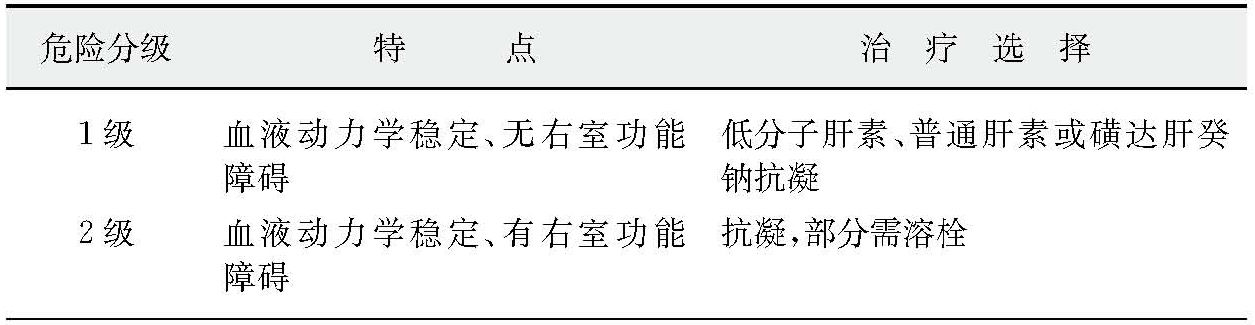
\includegraphics{./images/Image00129.jpg}
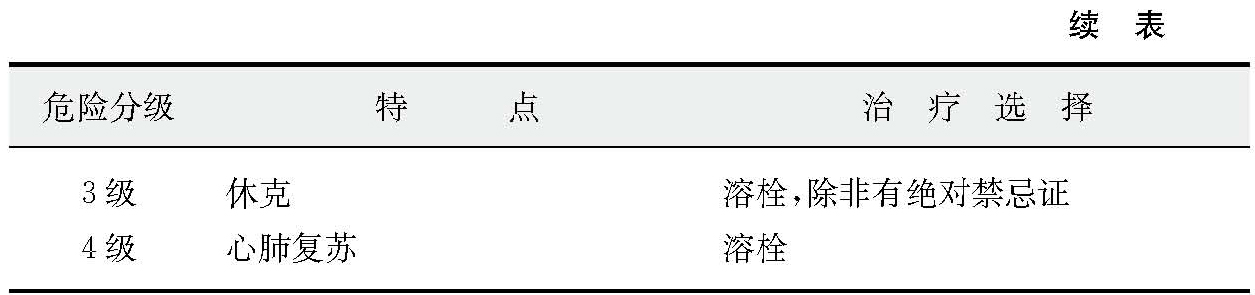
\includegraphics{./images/Image00130.jpg}
\end{table}



\subsubsection{次大面积肺血栓栓塞症是否应该溶栓?}

上述危险分层的指征中绝大多数都为血压正常但有右室功能障碍的次大面积或亚大面积肺血栓栓塞症,对此类患者进行溶栓的依据是:①右室功能障碍是影响预后的独立危险因素;②溶栓改善右室灌注可能有益于病情;③部分研究已证实以上临床受益。但目前为止,对次大面积肺血栓栓塞症的溶栓仍未达成共识。2002年Konstantinides等
\protect\hyperlink{text00022.htmlux5cux23ch21-21}{\textsuperscript{{[}21{]}}}
报道了256例急性肺血栓栓塞症伴肺动脉高压或右心室劳损患者的溶栓疗效报告。患者分为普通肝素+安慰剂组(138例)与普通肝素+组织型纤溶酶原激活物变异体溶栓组(118例),试验终点为死亡或治疗升级。治疗升级的定义为:应用血管活性药物提高血压、治疗后仍需溶栓、气管插管、心肺复苏及导管或手术摘除栓子。研究发现,普通肝素+安慰剂组病死率为2.2%,普通肝素+组织型纤溶酶原激活物变异体溶栓组为3.4%;复发率则分别为3.4%和2.9%,均无显著性差异,两组患者均未发生致命性出血,但普通肝素+安慰剂组死亡或治疗升级的风险比溶栓组高近3倍。由此,有学者认为次大面积肺血栓栓塞症不伴有血流动力学波动者,溶栓加抗凝可以改善预后,且溶栓治疗较为安全。

但该研究也引起了较多的争议。尽管病死率、复发率在统计学上没有显著性差异,抗凝组的年龄和基础疾病都显著高于溶栓组,因此无法证实溶栓治疗的有效性。因此次大面积或亚大面积肺血栓栓塞症是否需进行溶栓治疗尚需大样本的前瞻性研究。

\subsubsection{急性肺血栓栓塞症溶栓治疗荟萃分析的结论是什么?}

2004年的荟萃分析入选11项临床对照研究,共748例患者,发现由于入选病例数较少,疾病严重度与治疗异质性过大,溶栓与普通肝素抗凝在疗效上未有统计学差异。与普通肝素相比,溶栓治疗后肺血栓栓塞症的复发或死亡有降低趋势(6.7%对比9.6%;比值比0.67,95%CI0.40~1.12),大出血的发生率有增加趋势(9.1%对比6.1%,比值比1.42,95%CI0.81~2.46),但均无统计学差异。小量出血的发生率则显著增加(22.7%对比10.0%,比值比2.63,95%CI1.53~4.54)。

中国Cochrane进行的肺血栓栓塞症溶栓治疗的系统综述入选研究8项,总计患者679例,结论与2004年的荟萃分析相似。现有的证据不支持与抗凝相比,溶栓的病死率和复发率降低
\protect\hyperlink{text00022.htmlux5cux23ch22-21}{\textsuperscript{{[}22{]}}}
。因此需要更多的随机对照研究以评价溶栓治疗对于血液动力学稳定/不稳定的患者的效果。

\subsubsection{肺血栓栓塞症溶栓的原则是什么,如何监测及防治并发症?}

第8版国际抗凝与溶栓指南推荐对肺血栓栓塞症患者均进行危险分层评估,大部分患者不建议溶栓治疗。根据患者的临床表现和心功能受损情况进行分层,血流动力学不稳定或者休克患者的病死率高达58%,血流动力学稳定者则仅为15%。除非患者大出血并导致严重并发症,对于存在血流动力学不稳定的患者推荐立即溶栓。溶栓延迟可能发生顽固性的心源性休克。无低血压且出血风险较低的高危患者建议溶栓疗法。急性肺血栓栓塞症建议使用周围静脉而非肺动脉插管进行溶栓;建议短期滴注溶栓药物(如2小时),而非持续滴注(24小时)。对高出血风险或者一般状态很差的患者,在有经验医师和完善的设备的基础上,可考虑导管局部溶栓、导管取栓或手术取栓。

常用的溶栓药物有尿激酶、链激酶和组织型纤溶酶原激活物变异体,三者溶栓效果相似,临床上可根据患者选用。rt-PA对纤维蛋白具有选择性,溶栓作用强且快,半衰期短,减少了出血的不良反应,用药后不会发生过敏反应。而链激酶、尿激酶的特征是溶栓作用较强,但缺乏溶栓特异性,溶解纤维蛋白的同时也降解纤维蛋白原,易导致严重的出血。

①尿激酶 负荷量4400IU/kg静脉注射10分钟,随后以每小时2200IU/kg持续静脉滴注12小时;另可考虑2小时溶栓方案,即2万IU/kg尿激酶加入生理盐水100ml中持续静脉滴注2小时。

②链激酶 负荷量25万IU静脉注射30分钟,随后以10万IU/小时持续静脉滴注24小时。链激酶有抗原性,故用药前须肌肉注射苯海拉明或地塞米松防止过敏反应。

③rt-PA 50mg或100mg加入注射用水中持续静脉滴注2小时。

注射尿激酶、链激酶溶栓时勿同时应用普通肝素。溶栓治疗结束后,每2~4小时测定一次凝血酶原时间或部分凝血活酶时间,当其低于正常值的2倍时,可开始应用普通肝素抗凝。

北京朝阳医院组织的一项多中心随机对照前瞻性研究,研究纳入246例肺血栓栓塞症患者,应用不同的溶栓方案,发现尿激酶12小时组、尿激酶2小时组、组织型纤溶酶原激活物变异体50mg组及组织型纤溶酶原激活物变异体100mg组临床有效率分别为95.59%、94.34%、98.36%及94%。从临床疗效、安全性和经济效益等各方面综合考虑,使用50mg组织型纤溶酶原激活物变异体能获得更高的风险效益比,因此推荐应用组织型纤溶酶原激活物变异体50mg进行溶栓治疗方案。

溶栓治疗主要的并发症是出血,以颅内出血最为危险,发生率在0.3%~1.6%,尤易发生于老年人和有潜在出血危险的患者。入院时高舒张压是颅内出血的危险因素,一旦怀疑颅内出血,要立即停止溶栓治疗并请神经科医生会诊。此外,腹膜后血肿也是危险极大的并发症。溶栓后应动态观察临床表现及相关辅助检查,以评估溶栓的疗效及并发症。

\subsubsection{肺血栓栓塞症抗凝原则是什么,如何决定疗程?}

第8版国际抗凝与溶栓指南提出肺血栓栓塞症的抗凝原则,包括对于已证实的肺血栓栓塞症,推荐短期皮下注射低分子肝素、静脉或皮下注射普通肝素,或皮下注射磺达肝癸钠。急性肺血栓栓塞症患者应常规评估溶栓疗效。临床高度怀疑肺栓塞者,推荐在确诊的同时进行抗凝治疗。急性肺血栓栓塞症患者推荐应用低分子肝素、普通肝素或磺达肝癸钠治疗至少5天,直至国际标准化比值≥2.0超过24小时;维生素K拮抗剂与低分子肝素、普通肝素或磺达肝癸钠一起首日使用,而非推迟启用维生素K拮抗剂。肺血栓栓塞症抗凝治疗中,普通肝素、低分子肝素以及维生素K拮抗剂的初始治疗原则与下肢深静脉血栓基本相同。

抗凝治疗为肺静脉血栓栓塞症的基本治疗方法,其对已存在的血栓栓塞性疾病无治疗作用,但能有效防止血栓再形成和复发,同时机体的自身纤溶机制可以溶解已形成的血栓。目前临床上应用的抗凝药物主要有普通肝素、低分子肝素和华法林,在治疗初期先用普通肝素或低分子肝素,然后以华法林维持治疗。由于普通肝素和华法林存在着明显的副作用,且药效个体差异较大,需要连续监测,造成治疗的依从性差,目前逐渐被疗效更好、无需监测的新型抗凝药物所取代,如2004年第7次国际抗凝与溶栓会议制定的指南已推荐应用低分子肝素取代普通肝素(皮下注射或静脉滴注)作为下肢深静脉血栓和肺血栓栓塞症初始治疗的一线用药
\protect\hyperlink{text00022.htmlux5cux23ch1-21}{\textsuperscript{{[}1{]}}}
。

(1)肺血栓栓塞症的普通肝素抗凝治疗

普通肝素的禁忌证及用法 临床疑诊静脉血栓栓塞症时即可考虑使用普通肝素或低分子肝素进行抗凝治疗。应用普通肝素或低分子肝素前应测定部分凝血活酶时间、凝血酶原时间及血常规(含血小板计数、血红蛋白),观察是否存在抗凝的禁忌证。抗凝治疗的绝对禁忌证包括:①脑出血、消化系统出血急性期;②恶性肿瘤;③动(静)脉畸形。相对禁忌证包括:①既往有出血性疾病;②未控制的高血压(≥180/110mmHg);③2周内的大手术、创伤、活组织检查;④产后;⑤严重肝肾功能不全。

普通肝素的推荐用法为首剂予2000~5000IU或按80IU/kg静脉注射,继之以每小时18IU/kg持续静脉滴注。开始治疗后的24小时内每4~6小时测定部分凝血活酶时间,根据部分凝血活酶时间调整剂量,尽快使部分凝血活酶时间达到并维持于正常值的1.5~2.5倍。达稳定治疗目标后,每日测定部分凝血活酶时间1次。若抗凝不充分将严重影响疗效并可导致血栓的复发率增高。不推荐疗程中仅予静脉推注负荷剂量而无序贯给药,也不推荐不进行抗凝监测而盲目地抗凝治疗。

普通肝素亦可用皮下注射方式给药。推荐初始剂量是17500U,或者根据体重调整的剂量250IU/kg,每12小时皮下注射1次。同时根据部分凝血活酶时间调整普通肝素剂量,使注射后6~8小时的部分凝血活酶时间达到治疗目标。

普通肝素抗凝监测 普通肝素治疗常用的监测指标是部分凝血活酶时间。以静脉抗凝为例,监测部分凝血活酶时间的程序如表\ref{tab16-11}。\footnote{*在最初24小时,每6小时测定部分凝血活酶时间。随后可每天晨起测定部分凝血活酶时间1次,除非部分凝血活酶时间超标。}

\begin{table}[htbp]
\centering
\caption{普通肝素抗凝的监测与调整}
\label{tab16-11}
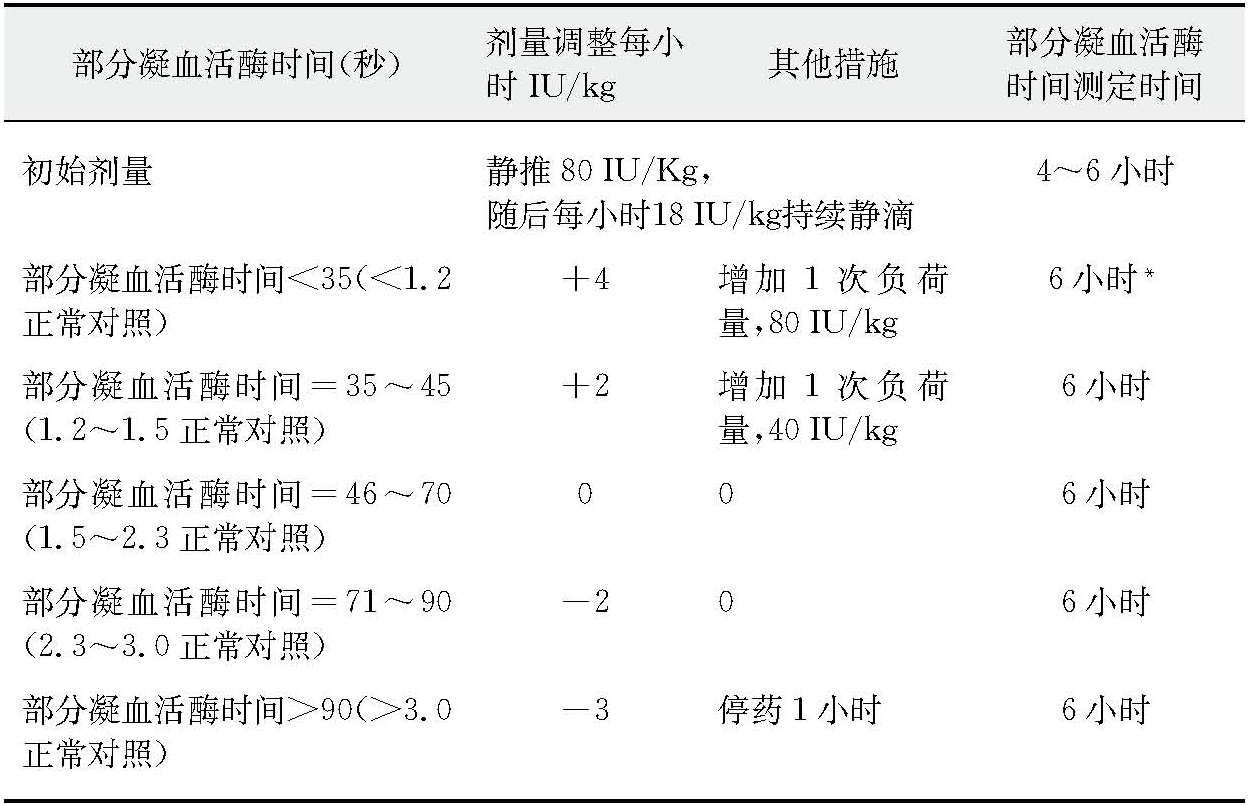
\includegraphics{./images/Image00131.jpg}
\end{table}



应用普通肝素过程中如大出血,出现皮肤淤斑、咯血、血尿或刺穿部位、胃肠道、阴道出血等,应监测血小板计数和其他凝血指标。普通肝素过量导致的出血,通常在停药后凝血功能即恢复,必要时可用硫酸鱼精蛋白对抗,即1mg鱼精蛋白对抗100IU普通肝素。普通肝素还可能引起血小板减少症,在使用普通肝素的第3~5天必须复查血小板计数。若需较长时间使用普通肝素,应在第7~10天和14天复查,血小板减少症很少于普通肝素治疗的2周后出现。若出现血小板迅速或持续降低30%,或血小板计数<100×10\textsuperscript{9}
/L,应停用普通肝素。一般在停用普通肝素后10天内血小板可逐渐恢复。须注意,血小板减少症可能会伴发静脉血栓栓塞症的进展或复发。当血栓复发的风险很大而又必须停用普通肝素时,可考虑放置下腔静脉滤器,但需警惕滤器处合并腔静脉血栓。

普通肝素与低分子肝素的比较 普通肝素远非理想的抗凝药。普通肝素可与内皮细胞或血浆蛋白中的凝血因子Ⅷ
、纤维蛋白酶原等结合,使普通肝素的生物活性下降;且个体之间剂量反应差异较大,甚至可能出现抗药现象。普通肝素与抗凝酶Ⅲ结合而成的复合物无法进入并激活凝血酶原复合物中的Xa,也无法接近与纤维蛋白结合的凝血酶,或无法到达内皮表面;同时,普通肝素对血小板功能有抑制作用,且影响血管的渗透性。以上特点导致普通肝素的应用受限,低分子肝素由普通肝素解聚分解而成,平均分子量为4000~6000道尔顿,与普通肝素相比,存在很多优点:①低分子肝素与血浆蛋白、内皮细胞和巨噬细胞结合较少,使其在较低剂量时就有良好的生物利用度和与剂量无关的廓清机制及较长的半衰期。因此,除肾功能障碍,或体重<50kg或>80kg的个体之外,低分子肝素监测次数较普通肝素减少。②低分子肝素的糖基较普通肝素的短,对Xa及凝血酶(尤其是Xa)的抑制作用强于普通肝素。③低分子肝素与血小板结合较少,抑制血小板功能弱于普通肝素,且低分子肝素不增加微血管的渗透性,与内皮细胞、血小板、Von-Wllebrand因子的亲和力低而较少引起出血。④低分子肝素与普通肝素在安全性与疗效上相似。荟萃分析发现,低分子肝素与普通肝素在血栓复发率、病死率、出血及血小板减少症等并发症上无统计学差异。⑤与口服华法林预防血栓复发相比,每日皮下注射一次低分子肝素效果相似,且出血等副作用较少,提示低分子肝素可用于存在出血风险的高危人群或难以实验室监测的患者。⑥低分子肝素无需实验室监测并可皮下注射,故广泛应用于门诊或住院的患者。⑦与普通肝素一样,低分子肝素对妊娠妇女也较安全,骨质疏松、血小板减少症的发生率较低,在应用低分子肝素的前5~7天亦无需监测血小板数量。

尽管低分子肝素存在如此多的优点,但其价格昂贵,且低分子肝素同样无法阻止凝血酶与纤维蛋白原的结合,因而限制了其临床应用。目前低分子肝素的品种较多,其用法用量各异,药效不一。

低分子肝素与普通肝素的局限性促进了新的抗凝药物的研发,包括磺达肝癸钠、水蛭素(hirudin)、因子Xa抑制剂、糖蛋白Iib/Ⅲa拮抗剂等。这些新药可以不依赖抗凝酶Ⅲ而直接抑制凝血酶或其他促凝物质的活性,使我们对血栓栓塞性疾病的防治有了质的飞跃。

(2)低分子肝素的用法 低分子肝素推荐根据体重给药,不同种低分子肝素的剂量不同,效价也不同,不能互相换算。一般用量为每日1~2次,皮下注射。对于大多数病例,按体重给药是有效的,不需监测部分凝血活酶时间和调整剂量,但对过度肥胖者或孕妇宜监测血浆抗Xa因子活性(plasma
anti-Xa activity)并据以调整剂量,目前上市的低分子肝素用法参见表\ref{tab16-12}。

\begin{table}[htbp]
\centering
\caption{低分子肝素用法与用量}
\label{tab16-12}
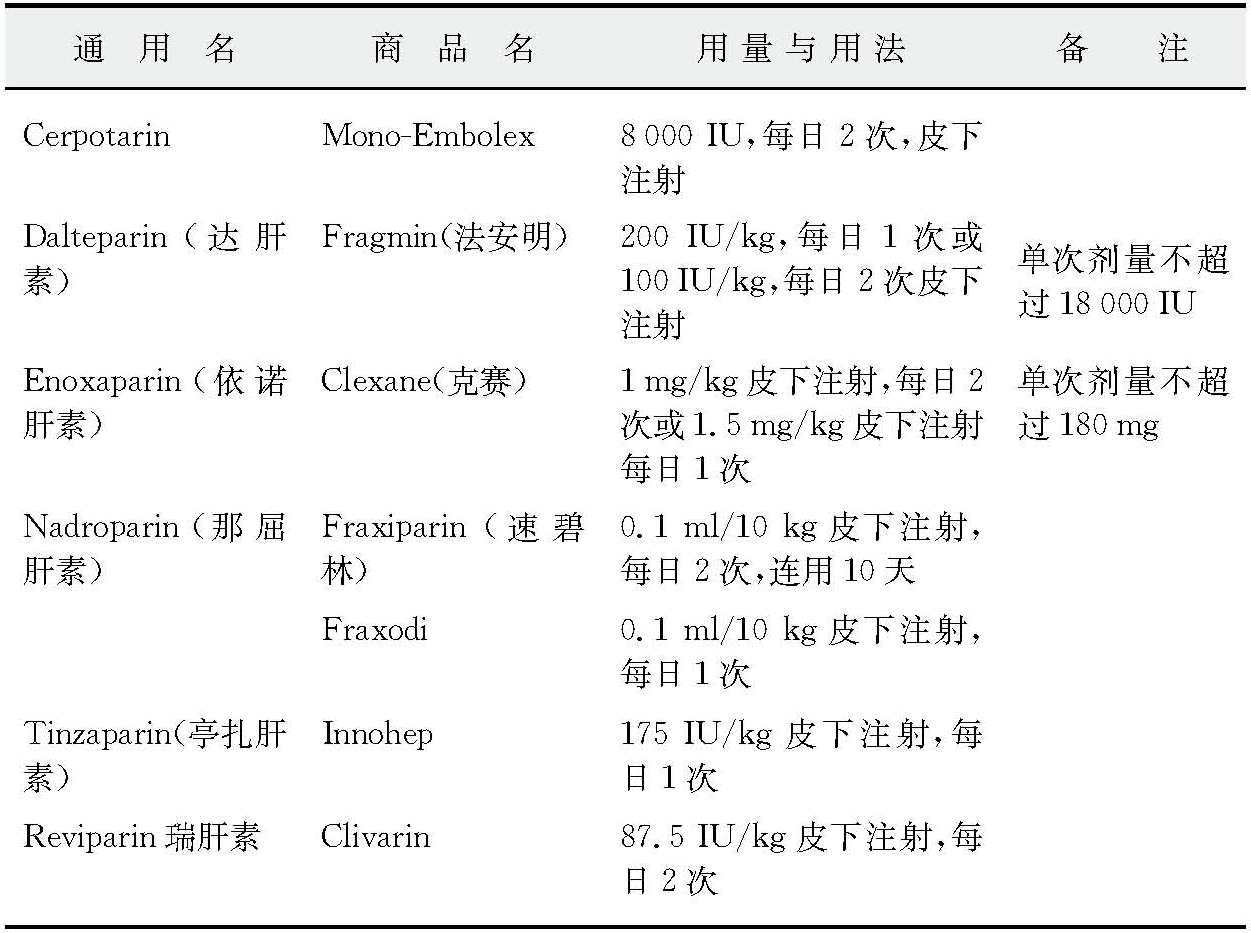
\includegraphics{./images/Image00133.jpg}
\end{table}

(3)抗凝治疗的临床应用报道与进展 对低分子肝素与普通肝素疗效比较的系统综述,纳入22项研究共8867例患者入选,主要结果见表\ref{tab16-13}。研究结论为低分子肝素在静脉血栓栓塞症的初始治疗中比普通肝素更为安全、更有效,病死率、血小板减少症发生率更低。

\begin{table}[htbp]
\centering
\caption{低分子肝素与普通肝素的Cochrane图书馆的系统综述}
\label{tab16-13}
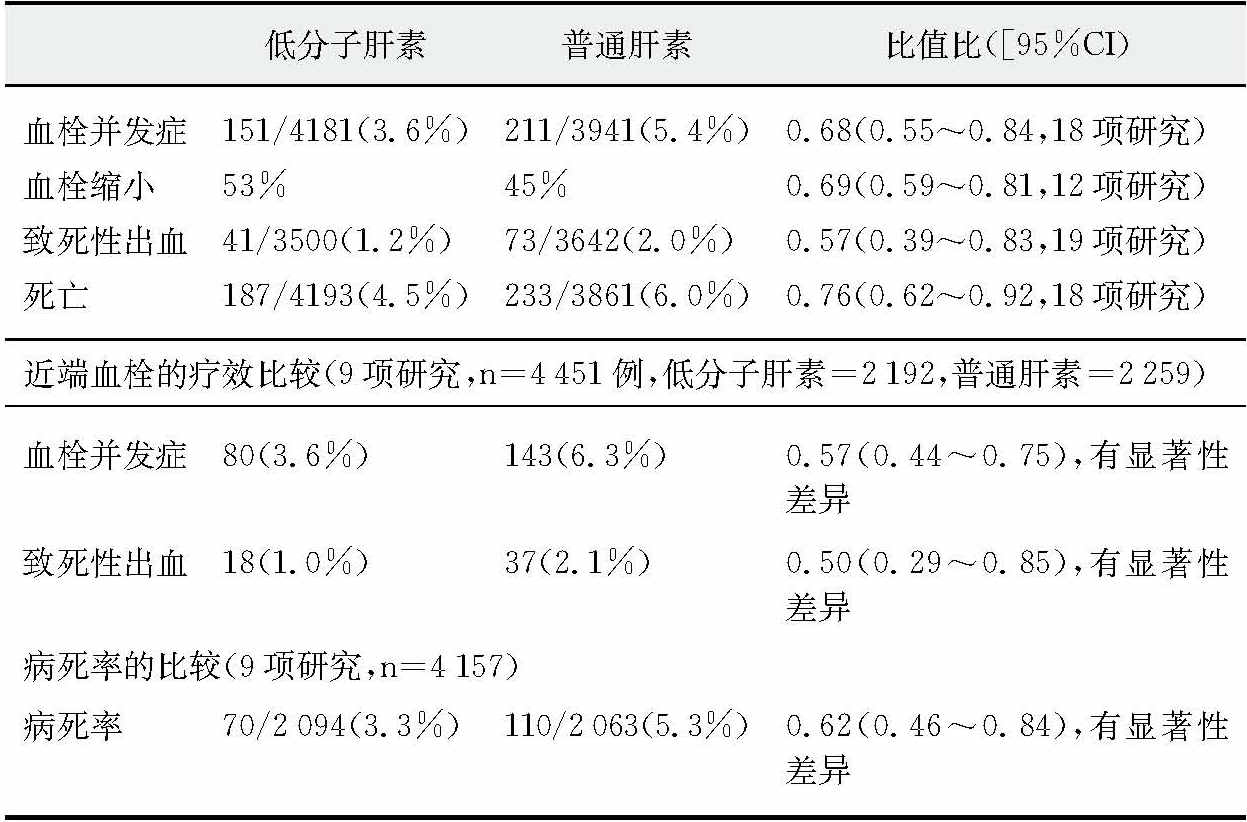
\includegraphics{./images/Image00134.jpg}
\end{table}

另有荟萃分析比较了低分子肝素每日1次与每日2次的疗法,共5项研究1508例患者入选。结果发现,单次用药血栓复发率和大出血发生率低于每日2次用药[比值比分别为0.82(0.49~1.39)和0.77(0.40~1.45)],而病死率稍高[比值比1.14(0.62~2.08)],但两者均无统计学差异。因此,尽管单次用药更易被患者接受,应用时仍需因人而异。

Wells报道了两种低分子肝素(达肝素与亭扎肝素)用于门诊静脉血栓栓塞症的前瞻性研究。患者在接受5天低分子肝素治疗的同时开始华法林治疗,之后华法林口服90天,研究纳入达肝素组254例,亭扎肝素251例。两组的血栓复发数分别为9例和10例,大出血分别为2例和5例,均无统计学差异,两药的疗效和安全性相似。

近年来,具有拮抗凝血因子Xa活性的新型抗凝药物磺达肝癸钠问世。该药皮下注射后能发挥其生物活性,体内不代谢,全部经肾脏排出;与低分子肝素一样,用药过程中不需要监测凝血指标。对2213例患者进行的对照研究(The
Matisse研究)应用5~10mg磺达肝癸钠每日1次皮下注射,5天疗程后华法林治疗3个月,发现磺达肝癸钠组与普通肝素组的血栓复发率分别为3.8%(42/1103)和5.0%(56/1110),大出血发生率分别为1.3%和1.1%,随访3个月后两组病死率也相似,分别为5.2%和4.4%。

针对磺达肝癸钠与低分子肝素(依诺肝素)在治疗下肢深静脉血栓方面的疗效比较显示,磺达肝癸钠组与低分子肝素组的血栓复发率分别为43/1098(3.9%)和45/1107(4.1%),大出血发生率分别为1.1%和1.2%;随访3个月两组的病死率也相似,分别为3.8%和3.0%。两项研究均证实磺达肝癸钠在静脉血栓栓塞症治疗方面的疗效与普通肝素和低分子肝素相似,为静脉血栓栓塞症的治疗提供了新的选择。目前,磺达肝癸钠已被美国FDA批准用于静脉血栓栓塞症的初始治疗或骨科矫形手术后静脉血栓栓塞症的预防,Ⅲ期临床试验证实磺达肝癸钠能使髋膝手术后静脉血栓栓塞症的风险下降55%,术后预防用药1~4周,通过静脉造影发现能使下肢深静脉血栓发生率由35%下降至1.4%,症状性静脉血栓栓塞症由2.7%下降至0.3%。

依达肝素作为磺达肝癸钠的超甲基化衍生物,与抗凝血酶具有超强的结合力,血浆半衰期达80小时,可每周1次皮下注射。Ⅱ期临床试验发现,其在治疗近端下肢深静脉血栓的疗效与出血的副作用方面与华法林相近,但该药不能用于肾衰竭患者,且此药同磺达肝癸钠一样不能被鱼精蛋白拮抗,对于此药物引起的大出血,可考虑使用重组Ⅶa因子。

希美加群(ximelagatran)是凝血酶抑制剂美拉加群(melagatran)的前体,是第一个口服凝血酶抑制剂,目前已在欧洲作为膝髋关节置换术后静脉血栓栓塞症的预防用药而上市,该药对预防静脉血栓栓塞症疗效较好,但其远期意义还不明确。副作用为转氨酶升高。

低分子肝素和磺达肝癸钠良好的药代学特性使其逐步取代普通肝素广泛应用于住院和门诊的静脉血栓栓塞症患者,但普通肝素的研究进展为其应用开拓了新的前景。Kearon等比较应用普通肝素和低分子肝素治疗急性静脉血栓栓塞症的疗效
\protect\hyperlink{text00022.htmlux5cux23ch23-21}{\textsuperscript{{[}23{]}}}
。研究中应用333IU/kg的负荷量皮下注射普通肝素,继之250IU/kg,每日2次皮下注射。低分子肝素为达肝素或依诺肝素100IU/kg,每日2次皮下注射。随后两组均转为华法林口服3个月。两组的血栓复发率分别为3.8%和3.4%;治疗10天内大出血的发生率分别为1.1%和1.4%。该研究根据体重给药,普通肝素组未监测部分凝血活酶时间,且72%为门诊患者;低分子肝素组约68%为门诊患者,首次证实按体重皮下给药方式可将普通肝素应用于门诊患者,且其疗效与低分子肝素相当,治疗费用也明显降低。由此看来,部分凝血活酶时间监测可能并非普通肝素治疗所必需,但仍需更多研究支持。

第8版国际抗凝与溶栓指南指出,对于急性非大面积肺血栓栓塞症,推荐给予低分子肝素作为初始治疗。而对于急性大面积肺血栓栓塞症患者,由于皮下注射可能影响药物吸收以及患者可能同时进行溶栓治疗,静脉注射普通肝素更被推荐。对于接受低分子肝素治疗的急性肺血栓栓塞症患者,不推荐常规监测抗Xa因子水平。对于合并严重肾衰竭的急性肺血栓栓塞症的患者,相比低分子肝素,更推荐应用普通肝素。

\subsubsection{怎样确定华法林口服的疗程,如何监测?}

可在普通肝素或低分子肝素开始应用后的第1~3天加用口服抗凝剂华法林,初始剂量为3.0~5.0mg/天。由于华法林需要数天才能发挥全部作用,因此需与普通肝素或低分子肝素重叠4天以上,当连续2天测定的国际标准化比值达2.5(2.0~3.0),或凝血酶原时间延长至1.5~2.5倍时,可停用普通肝素或低分子肝素,单独口服华法林治疗。以后根据国际标准化比值或凝血酶原时间调节华法林的剂量。在达治疗目标前,应每日测定国际标准化比值,达标后两周每周监测2~3次,然后根据国际标准化比值的情况减少监测1次数。若长期治疗,每月需测定国际标准化比值并调整华法林剂量。

针对维生素K拮抗剂的抗凝强度,第8版国际抗凝与溶栓指南建议肺血栓栓塞症患者在治疗期间调整维生素K拮抗剂剂量使目标国际标准化比值为2.5(2.0~3.0)。对不明原因(unprovoked)的肺血栓栓塞症患者,在3个月的传统强度的抗凝治疗之后(国际标准化比值2.0~3.0),推荐低强度治疗(国际标准化比值1.5~1.9),不推荐采用高强度维生素K拮抗剂治疗(国际标准化比值3.1~4.0)。

根据第8版国际抗凝与溶栓指南,抗凝治疗的时间因人而异。对于可逆的肺血栓栓塞症患者,推荐维生素K拮抗剂治疗3个月;对不明原因肺血栓栓塞症,推荐维生素K拮抗剂治疗至少3个月(1A),所有患者均需进行长期治疗的风险---获益比评估。如首次发生的静脉血栓栓塞症是肺血栓栓塞症,并能够实施抗凝监测,推荐长期治疗。无症状性的肺血栓栓塞症一经发现,进行与症状性肺血栓栓塞症相同的初始和长期治疗。用药期间应定期评估出血风险、复发风险以及患者的临床表现。由于血栓后综合征多于下肢深静脉血栓两年后出现,可以选择穿戴弹力袜,保持踝部压力为30~40mmHg,可使血栓后综合征的发生率减少50%~60%。

\subsubsection{应用维生素K拮抗剂华法林治疗的患者应该注意什么?}

(1)对华法林代谢有影响的药物及食物 ①使华法林抗凝作用增强的药物有乙酰水杨酸、苯基丁氮酮、西咪替丁、D860、奎尼丁、丙咪嗪、头孢哌酮、头孢唑林、头孢噻吩、头孢曲松、红霉素、甲硝唑、磺胺类、环丙沙星、氧氟沙星、四环素、氟康唑、伊曲康唑、胺碘酮、普罗帕酮、三环类抗抑郁药、维生素E、丹参、当归等。②使华法林抗凝作用减弱的药物有苯妥英钠、苯巴比妥、维生素K、利福平、安体舒通、卡马西平、硫糖铝、人参、辅酶Q10、抗甲状腺素药物等。

(2)致畸作用 华法林可透过胎盘,孕期妇女接受华法林治疗可导致胎儿严重的骨骼发育异常,故禁用于妊娠妇女。分娩后母乳中华法林代谢物不具有抗凝作用,可用华法林治疗。尚无证据表明成人或儿童应用华法林会直接影响骨代谢。

(3)出血 华法林剂量过大或国际标准化比值>3.0时易发生出血,发生率6%。轻中度出血者可用维生素K拮抗剂治疗。

(4)疗程 华法林疗程一般为6个月~1年,对于存在高易患因素的肺血栓栓塞症,如合并恶性肿瘤或复发性静脉血栓栓塞症,且并发肺心病或肺动脉高压者,需长期或终身抗凝治疗。

\subsubsection{肺血栓栓塞症的介入治疗方法有哪些?}

(1)导管取栓术 大块血栓所致肺血栓栓塞症急性期病死率达32%,发病1小时内病死率达11%,故对于大面积肺血栓栓塞症患者,介入治疗是迅速改善呼吸循环障碍的有效方法。介入治疗适应证为:①急性大面积肺血栓栓塞症;②存在溶栓禁忌证或经溶栓治疗无效;③人工心肺支持禁忌或无法实施。此外,介入治疗的成功还取决于训练有素的治疗队伍。

德国报道了204家医疗中心1001例应用碎栓术治疗大面积肺血栓栓塞症的研究,发现合并右室功能障碍者占1.7%,低血压者占1.3%,心源性休克者占2.9%,循环障碍者占6.8%;且症状愈重,导管治疗的实施率愈高。接受介入检查和治疗的院内病死率为11%,而未能积极检查和治疗者院内病死率达45%,提示急性大面积肺血栓栓塞症采用介入治疗的重要性。发病初期病情危重的肺血栓栓塞症患者,如能渡过急性期则预后较好,早期介入治疗对改善患者病情和维持血流动力学稳定有较大意义。

(2)下腔静脉滤器置入 置入滤器的目的是预防静脉内的大块栓子脱落和肺血栓栓塞症的复发,其对已经形成的血栓不产生任何治疗作用,接受滤器置入的患者需要尽早充分抗凝。一项研究报道了对永久性滤器置入患者的8年随访结果,发现尽管滤器能够减少肺血栓栓塞症的发生(置入组与非置入组肺血栓栓塞症发生率分别为6.2%对比15.1%,\emph{P}
=0.008),但下肢深静脉血栓的发生率却有所增加(35.7%对比27.5%,\emph{P}
=0.042),且滤器置入组血栓后综合征以及病死率有升高趋势,但无显著性差异。2006年临时性滤器置入的国际共识颁布
\protect\hyperlink{text00022.htmlux5cux23ch24-21}{\textsuperscript{{[}24{]}}}
,认为滤器不适合常规用于静脉血栓栓塞症的治疗,如需置入,首选临时性滤器,且待病因消除后须将滤器取出。

第8版国际抗凝与溶栓指南提出除抗凝治疗外,大多肺血栓栓塞症患者不推荐常规使用腔静脉滤器。存在出血风险而无法使用抗凝剂的急性肺血栓栓塞症患者,推荐放置下腔静脉滤器;已置入下腔静脉滤器替代抗凝治疗急性肺血栓栓塞症患者,一旦出血风险解决,应接受传统的抗凝治疗。

\subsubsection{肺血栓栓塞症的外科治疗指征是什么?}

急性大面积肺血栓栓塞症经溶栓或导管碎栓术等方法无效时可考虑肺动脉直接取栓术,但此手术风险较大,病死率高。第8版国际抗凝与溶栓指南推荐对某些严重失代偿且因岀血无法接受溶栓治疗或病情危急没有充分的时间进行全身溶栓的患者,在条件具备的情况下可施行栓子切除术。

\subsubsection{慢性血栓栓塞性肺动脉高压有哪些治疗方法?}

急性肺血栓栓塞症发展为慢性血栓栓塞性肺动脉高压者占0.1%~3.8%。慢性血栓栓塞性肺动脉高压为肺动脉内反复栓塞及血栓形成致肺血管阻力增加,表现为血栓栓塞性肺动脉高压及右室功能障碍,发病多隐匿、缓慢。内科多为对症治疗,无特异治疗方法:①抗凝治疗,防止新血栓的形成和肺血栓栓塞症的再发,遏制肺动脉高压进展,且可能促进血栓溶解再通。常用药物包括华法林等抗凝剂,剂量为3.0~5.0mg/天,根据国际标准化比值调整剂量,疗程至少6个月,停药后若症状加重可继续应用。②血管扩张剂,用于降低肺动脉压力,临床上可以应用前列腺素E、一氧化氮、钙离子拮抗剂、酚妥拉明等,也可服用抗血小板聚集药。③治疗右心衰,有明显右心衰时应使用强心剂、利尿剂或血管紧张素转换酶抑制剂等。

如病情允许,可考虑外科行肺动脉切开取栓术、肺动脉内膜剥脱术和双侧肺移植术。第8版国际抗凝与溶栓指南提出对所有慢性血栓栓塞性肺动脉高压患者,建议终身服用维生素K拮抗剂抗凝,将国际标准化比值控制在2.0~3.0。部分患者(如中心型)在经验丰富的医疗团队治疗,可考虑行肺动脉血栓内膜剥脱术,术前或术中可考虑置入腔静脉滤器。

\subsubsection{静脉血栓栓塞症如何预防?}

静脉血栓栓塞症的预防是系统工程,涉及门诊和住院的危险度各不相同的患者,因此选择的预防手段以及疗程各不相同,表\ref{tab16-14}是根据第7次抗凝与溶栓会议的共识建立的静脉血栓栓塞症预防策略。

\begin{table}[htbp]
\centering
\caption{预防静脉血栓栓塞症的策略}
\label{tab16-14}
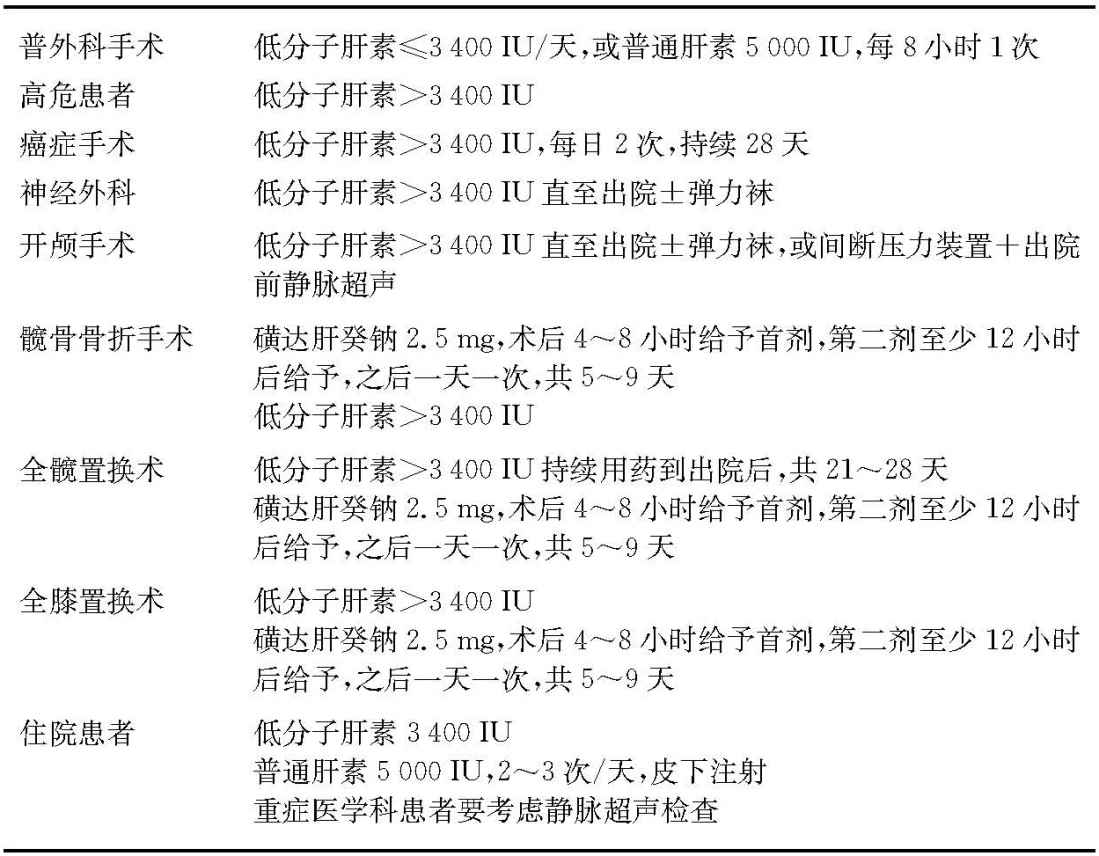
\includegraphics{./images/Image00135.jpg}
\end{table}

总之,随着现代医疗技术的进步与发展,对静脉血栓栓塞症发病机制的认识也日趋深入,基于循证医学证据的诊断、治疗和预防指南也不断出台,规范性诊治取得了显著进步,患者的存活率和生存质量明显提高。但下肢深静脉血栓和肺血栓栓塞症领域仍然有诸多问题等待进一步的解决,如最佳诊断策略、区域化或个体化诊疗策略的制定、次大面积肺血栓栓塞症溶栓治疗以及特定人群的流行病学和预防策略等都值得关注。相信随着越来越多的证据的出现,静脉血栓栓塞症的诊治水平会进入新的阶段,我们也期望国内学者能早日开展有中国特色的高水平的研究,为切实降低静脉血栓栓塞症的病死率、致残率做出贡献。

\begin{center}\rule{0.5\linewidth}{\linethickness}\end{center}

参考文献

\protect\hyperlink{text00022.htmlux5cux23ch1-21-back}{{[}1{]}} .Buller
HR,Agnelli G,Hull RD,et al.Antithrombotic therapy for venous
thromboembolic disease:the Seventh ACCP Conference on Antithrombotic
and Thrombolytic Therapy.Chest,2004,126:S401-S428.

\protect\hyperlink{text00022.htmlux5cux23ch2-21-back}{{[}2{]}} .Dalen
JE.Pulmonary Embolism:What Have We Learned Since Virchow?Treatment
and Prevention.Chest,2002,122:1801-1817.

\protect\hyperlink{text00022.htmlux5cux23ch3-21-back}{{[}3{]}} .Michota
F.Venous thromboembolism epidemiology,Characteristics,and
Consequences.Clinc Cornerstone,2005,7:8-15.

\protect\hyperlink{text00022.htmlux5cux23ch4-21-back}{{[}4{]}}
.Velmahaos G.The current status of thromboprophylaxis after Truma:a
story of confusion and uncertainty.Am Surg,2006,72:757-763.

\protect\hyperlink{text00022.htmlux5cux23ch5-21-back}{{[}5{]}} .Blann
AD,Lip GYH.Venous thromboembolism.BMJ,2006,332:215-219.

{[}6{]}.Goldhaber SZ.Pulmonary
embolism.Lancet,2004,363:1295-1305.

\protect\hyperlink{text00022.htmlux5cux23ch7-21-back}{{[}7{]}} .Wheeler
A.Venous thromboembolism in medically ill patients identifying risk and
strategies for prevention.Clinc Cornerstone,2005,7:23-31.

\protect\hyperlink{text00022.htmlux5cux23ch8-21-back}{{[}8{]}} .Wells
P.Advances in the diagnosis of venous thromboembolism.J Thromb
Thrombolysis,2006,21:31-40.

\protect\hyperlink{text00022.htmlux5cux23ch9-21-back}{{[}9{]}} .Motsch
J,Walther A,Bock M,et al.Update in the prevention and treatment of
deep vein thrombosis and pulmonary embolism.Curr Opin
Anaesthesiol,2006,19:52-58.

\protect\hyperlink{text00022.htmlux5cux23ch10-21-back}{{[}10{]}}
.Moores LK,King CS,Holley AB.Current Approach to the Diagnosis of
Acute Nonmassive Pulmonary Embolism.Chest,2011,140:509-518.

\protect\hyperlink{text00022.htmlux5cux23ch11-21-back}{{[}11{]}}
.Konstantinides S,Geibel A,Olschewski M,et al.Importance of cardiac
troponins I and T in risk stratification of patients with acute
pulmonary embolism.Circulation,2002,106:1263-1268.

\protect\hyperlink{text00022.htmlux5cux23ch12-21-back}{{[}12{]}}
.Kucher N,Printzen G,Doernhoefer T,et al.Low pro-brain natriuretic
peptide levels predict benign clinical outcome in acute pulmonary
embolism.Circulation,2003,107:1576-1578.

\protect\hyperlink{text00022.htmlux5cux23ch13-21-back}{{[}13{]}}
.PIOPED Investigators.Value of the ventilation/perfusion scan in acute
pulmonary embolism.JAMA,1990,263:2753-2759.

\protect\hyperlink{text00022.htmlux5cux23ch14-21-back}{{[}14{]}}
.Morris TA,Marsh JJ,Chiles PG,et al.Single photon emission computed
tomography of pulmonary emboli and venous thrombi using anti-D-dimer.Am
J Respir Crit Care Med,2004,169:987-993.

\protect\hyperlink{text00022.htmlux5cux23ch15-21-back}{{[}15{]}} .Stein
PD,Fowler SE,Goodman LR,et al.Multidetector computed tomography for
acute pulmonary embolism.N Engl J Med,2006,354:2317-2327.

\protect\hyperlink{text00022.htmlux5cux23ch16-21-back}{{[}16{]}} .Hogg
K,Brown G,Dunning J,et al.Diagnosis of pulmonary embolism with CT
pulmonary angiography:a systematic review.Emerg Med
J,2006,23:172-178.

\protect\hyperlink{text00022.htmlux5cux23ch17-21-back}{{[}17{]}}
.Quiroz R,Kucher N,Zou KH,et al.Clinical validity of a negative
computed tomography scan in patients with suspected pulmonary
embolism:a systematic review.JAMA,2005,293:2012-2017.

\protect\hyperlink{text00022.htmlux5cux23ch18-21-back}{{[}18{]}} .Stein
PD,Chenevert TL,Fowler SE,et al.Gadolinium-enhanced magnetic
resonance angiography for pulmonary embolism:a multicenter prospective
study(PIOPED Ⅲ).Ann Intern Med,2010,152:34-43.

\protect\hyperlink{text00022.htmlux5cux23ch19-21-back}{{[}19{]}}
.Kearon C,Kahn SR,Agnelli G,et al.Antithrombotic therapy for venous
thromboembolic disease:American College of Chest Physicians
Evidence-Based Clinical Practice Guidelines(8th
Edition).Chest,2008,133(6 Suppl):454S-545S.

\protect\hyperlink{text00022.htmlux5cux23ch20-21-back}{{[}20{]}}
.Watson LI,Armon MP.Thrombolysis for acute deep vein
thrombosis.Cochrane Database Syst Rev,2004,18:CD002783.

\protect\hyperlink{text00022.htmlux5cux23ch21-21-back}{{[}21{]}}
.Konstantinides S,Geibel A,Heusel G,et al.Heparin plus alteplase
compared with heparin alone in patients with submassive pulmonary
embolism.N Engl J Med,2002,347:1143-1150.

\protect\hyperlink{text00022.htmlux5cux23ch22-21-back}{{[}22{]}} .Dong
B,Jirong Y,Liu G,et al.Thrombolytic therapy for pulmonary
embolism.Cochrane Database Syst Rev,2006,19:CD004437.

\protect\hyperlink{text00022.htmlux5cux23ch23-21-back}{{[}23{]}}
.Kearon C,Ginsberg JS,Julian JA,et al.Comparison of fixed-dose
weight-adjusted unfractionated heparin and low-molecular-weight heparin
for acute treatment of venous
thromboembolism.JAMA,2006,296:935-942.

\protect\hyperlink{text00022.htmlux5cux23ch24-21-back}{{[}24{]}}
.Kaufman JA,Kinney TB,Streiff MB,et al.Guidelines for the use of
retrievable and convertible vena cava filters:report from the Society
of Interventional Radiology multidisciplinary consensus conference.J
Vasc Interv Radiol,2006,17:449-459.

\protect\hypertarget{text00023.html}{}{}

